%%%%%%%%%%%%%%%%%%%%%%%%%%%%%%% beamer %%%%%%%%%%%%%%%%%%%%%%%%%%%%%%%%%%%%%%%%%%%%%%%%%
% To run - pdflatex filename.tex
%	   acroread filename.pdf
%%%%%%%%%%%%%%%%%%%%%%%%%%%%%%%%%%%%%%%%%%%%%%%%%%%%%%%%%%%%%%%%%%%%%%%%%%%%%%%%%%%%%%%%

\documentclass[compress,red]{beamer}
\mode<presentation>
\setbeamertemplate{navigation symbols}{}

\usetheme{Warsaw}
% other themes: AnnArbor, Antibes, Bergen, Berkeley, Berlin, Boadilla, boxes, CambridgeUS, Copenhagen, Darmstadt, default, Dresden, Frankfurt, Goettingen,
% Hannover, Ilmenau, JuanLesPins, Luebeck, Madrid, Maloe, Marburg, Montpellier, PaloAlto, Pittsburg, Rochester, Singapore, Szeged, classic

%\usecolortheme{lily}
% color themes: albatross, beaver, beetle, crane, default, dolphin, dov, fly, lily, orchid, rose, seagull, seahorse, sidebartab, structure, whale, wolverine

%\usefonttheme{serif}
% font themes: default, professionalfonts, serif, structurebold, structureitalicserif, structuresmallcapsserif

\hypersetup{pdfpagemode=FullScreen} % makes your presentation go automatically to full screen

% define your own colors:
\definecolor{Red}{rgb}{1,0,0}
\definecolor{Blue}{rgb}{0,0,1}
\definecolor{Green}{rgb}{0,1,0}
\definecolor{magenta}{rgb}{1,0,.6}
\definecolor{lightblue}{rgb}{0,.5,1}
\definecolor{lightpurple}{rgb}{.6,.4,1}
\definecolor{gold}{rgb}{.6,.5,0}
\definecolor{orange}{rgb}{1,0.4,0}
\definecolor{hotpink}{rgb}{1,0,0.5}
\definecolor{newcolor2}{rgb}{.5,.3,.5}
\definecolor{newcolor}{rgb}{0,.3,1}
\definecolor{newcolor3}{rgb}{1,0,.35}
\definecolor{darkgreen1}{rgb}{0, .35, 0}
\definecolor{darkgreen}{rgb}{0, .6, 0}
\definecolor{darkred}{rgb}{.75,0,0}

\xdefinecolor{olive}{cmyk}{0.64,0,0.95,0.4}
\xdefinecolor{purpleish}{cmyk}{0.75,0.75,0,0}

% can also choose different themes for the "inside" and "outside"

% \usepackage{beamerinnertheme_______}
% inner themes include circles, default, inmargin, rectangles, rounded

% \usepackage{beamerouterthemesmoothbars}
% outer themes include default, infolines, miniframes, shadow, sidebar, smoothbars, smoothtree, split, tree

\useoutertheme[subsection=false]{smoothbars}

% to have the same footer on all slides
%\setbeamertemplate{footline}[text line]{STUFF HERE!}
\setbeamertemplate{footline}[text line]{} % makes the footer EMPTY

%To generate note pages after each slide
%\setbeameroption{show notes}

% include packages
\usepackage{subfigure}
\usepackage{multicol}
\usepackage{amsmath}
\usepackage{epsfig}
\usepackage{graphicx}
\usepackage[all,knot]{xy}
\xyoption{arc}
\usepackage{url}
\usepackage{multimedia}
\usepackage{hyperref}
\usepackage{helvet}
     
%%%%%%%%%%%%%%%%%%%%%%%%%%%%%%%%%%%%%%%%%%%%%%%%%%%%%%%%%%%%%%%%%%%%%%%%%%%%%%%%%%%%%%%%%%
%%%%%%%%%%%%%%%%%%%%%%%%%%%%%% Title Page Info %%%%%%%%%%%%%%%%%%%%%%%%%%%%%%%%%%%%%%%%%%%
%%%%%%%%%%%%%%%%%%%%%%%%%%%%%%%%%%%%%%%%%%%%%%%%%%%%%%%%%%%%%%%%%%%%%%%%%%%%%%%%%%%%%%%%%%
% Guidelines
% CERN 2'
% General arch 3'
% Open hardware 15'
% White Rabbit 10'
% FMC HW and HDL flow incl. WB 5'
% Software incl WB and ZIO 15'


\title{A strategy for managing diverse equipment in the CERN controls group}
%\subtitle{Update on specifications}
\author[Javier Serrano, David Cobas et al.]{Javier Serrano, Juan David
Gonz\'alez Cobas}
%\institute{CERN\\Geneva, Switzerland}
\date{FOSDEM 2012}

%%%%%%%%%%%%%%%%%%%%%%%%%%%%%%%%%%%%%%%%%%%%%%%%%%%%%%%%%%%%%%%%%%%%%%%%%%%%%%%%%%%%%%%%%%
%%%%%%%%%%%%%%%%%%%%%%%%%%%%%% Begin Your Document %%%%%%%%%%%%%%%%%%%%%%%%%%%%%%%%%%%%%%%
%%%%%%%%%%%%%%%%%%%%%%%%%%%%%%%%%%%%%%%%%%%%%%%%%%%%%%%%%%%%%%%%%%%%%%%%%%%%%%%%%%%%%%%%%%
%\useoutertheme{smoothbars}
\setbeamertemplate{footline}[page number]

\begin{document}

%%%%%%%%%%%%%%%%%%%%%%%%%%%%%%%%%%%%%%%%%%%%%%%%%%%%%%%%%%%%%%%%%%%%%%%%%%%%%%%%%%%%%%%%%%

\frame{
	\titlepage 
%\hfill {\footnotesize With help from Steve Smith (SLAC)}
}

%%%%%%%%%%%%%%%%%%%%%%%%%%%%%%%%%%%%%%%%%%%%%%%%%%%%%%%%%%%%%%%%%%%%%%%%%%%%%%%%%%%%%%%%%%
\AtBeginSubsection[] % Do nothing for \section*
{
\begin{frame}<beamer>
\frametitle{Outline}
\tableofcontents[currentsection, currentsubsection]
\end{frame}
}

%\section[Outline]{}	% this puts the outline before EACH section automatically & will highlight the section you're about to talk about


\frame{\tableofcontents}

%%%%%%%%%%%%%%%%%%%%%%%%%%%%%%%%%%%%%%%%%%%%%%%%%%%%%%%%%%%%%%%%%%%%%%%%%%%%%%%%%%%%%%%%%%
\section{Intro to CERN}
%%%%%%%%%%%%%%%%%%%%%%%%%%%%%%%%%%%%%%%%%%%%%%%%%%%%%%%%%%%%%%%%%%%%%%%%%%%%%%%%%%%%%%%%%%

\subsection{Particle accelerators: why?}

\frame{
\frametitle{Find out about what the world is made of...}
%\framesubtitle {}
\begin{center}
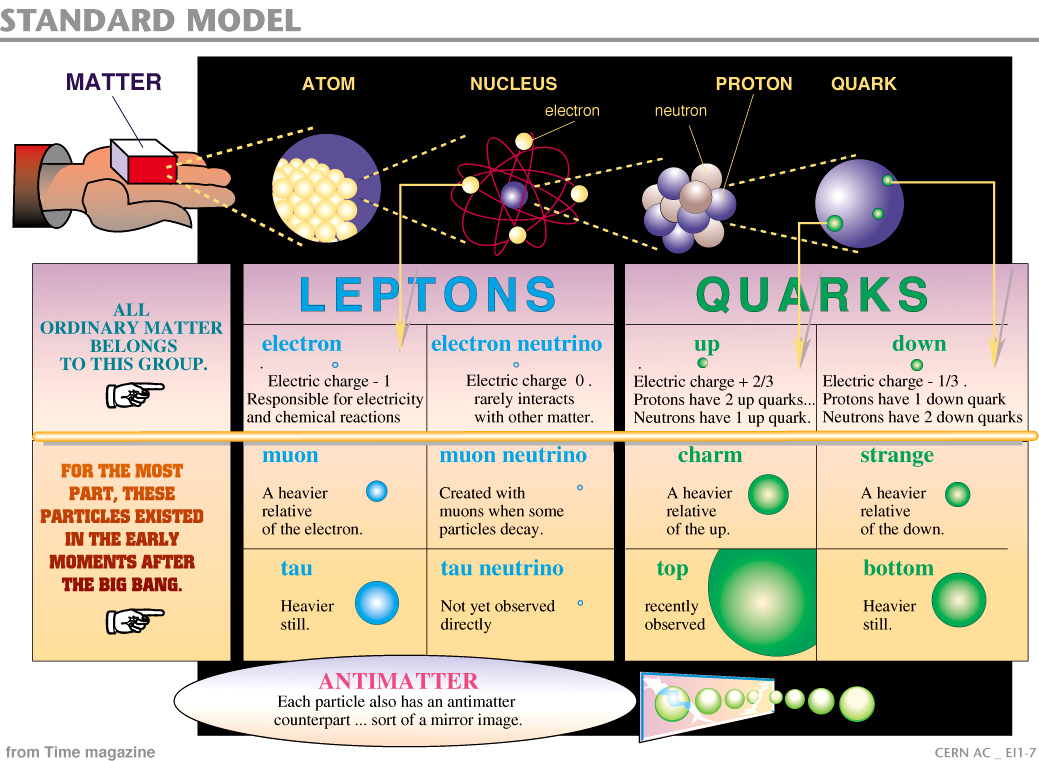
\includegraphics[width=.95\textwidth, height=0.8\textheight, keepaspectratio]{standard_model.jpg}
\end{center}
}

\frame{
\frametitle{\ldots and what other worlds might be made of!}
%\framesubtitle {}
\begin{center}
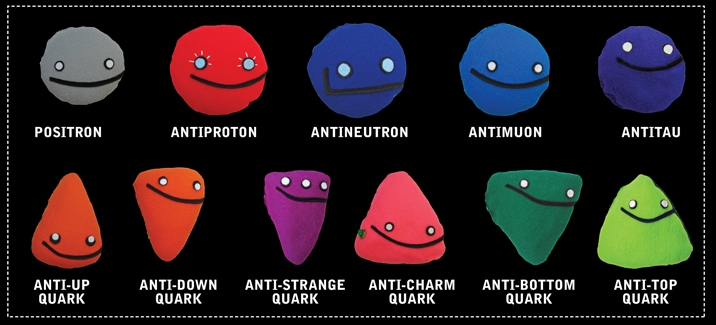
\includegraphics[width=.95\textwidth, height=0.8\textheight, keepaspectratio]{antiparticles.jpg}
\end{center}
}

\frame{
\frametitle{Better microscopes for biologists and other scientists}
%\framesubtitle {E.g. Mouse brain to study Alzheimer}
\begin{center}
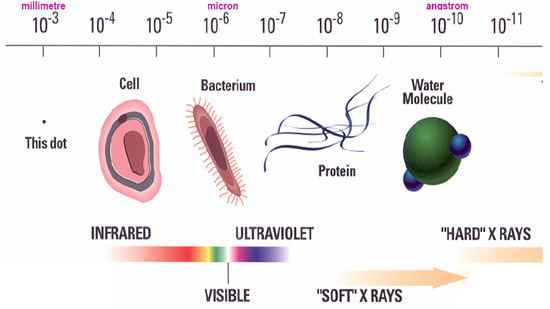
\includegraphics[width=.95\textwidth, height=0.8\textheight, keepaspectratio]{syn_light.jpg}
\end{center}
}

\frame{
\frametitle{Better microscopes for biologists and other scientists}
\framesubtitle {E.g. Mouse brain to study Alzheimer}
\begin{center}
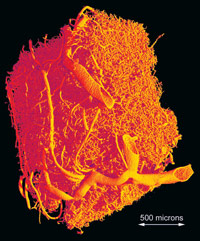
\includegraphics[width=.95\textwidth, height=0.8\textheight, keepaspectratio]{mouse_brain.jpg}
\end{center}
}

\frame{
\frametitle{Better microscopes for biologists and other scientists}
\framesubtitle {E.g. Nucleosome core}
\begin{center}
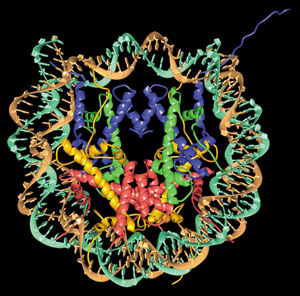
\includegraphics[width=.95\textwidth, height=0.8\textheight, keepaspectratio]{nucleosome_core.jpg}
\end{center}
}

\frame{
\frametitle{Fight tumors more effectively}
\framesubtitle {Hadron therapy}
\begin{center}
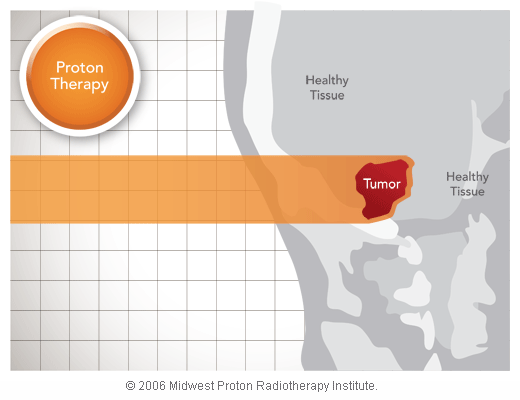
\includegraphics[width=.95\textwidth, height=0.8\textheight, keepaspectratio]{tumor.png}
\end{center}
}

\frame{
\frametitle{Fight tumors more effectively}
\framesubtitle {Better energy deposition than X-rays and traditional radiotherapy}
\begin{center}
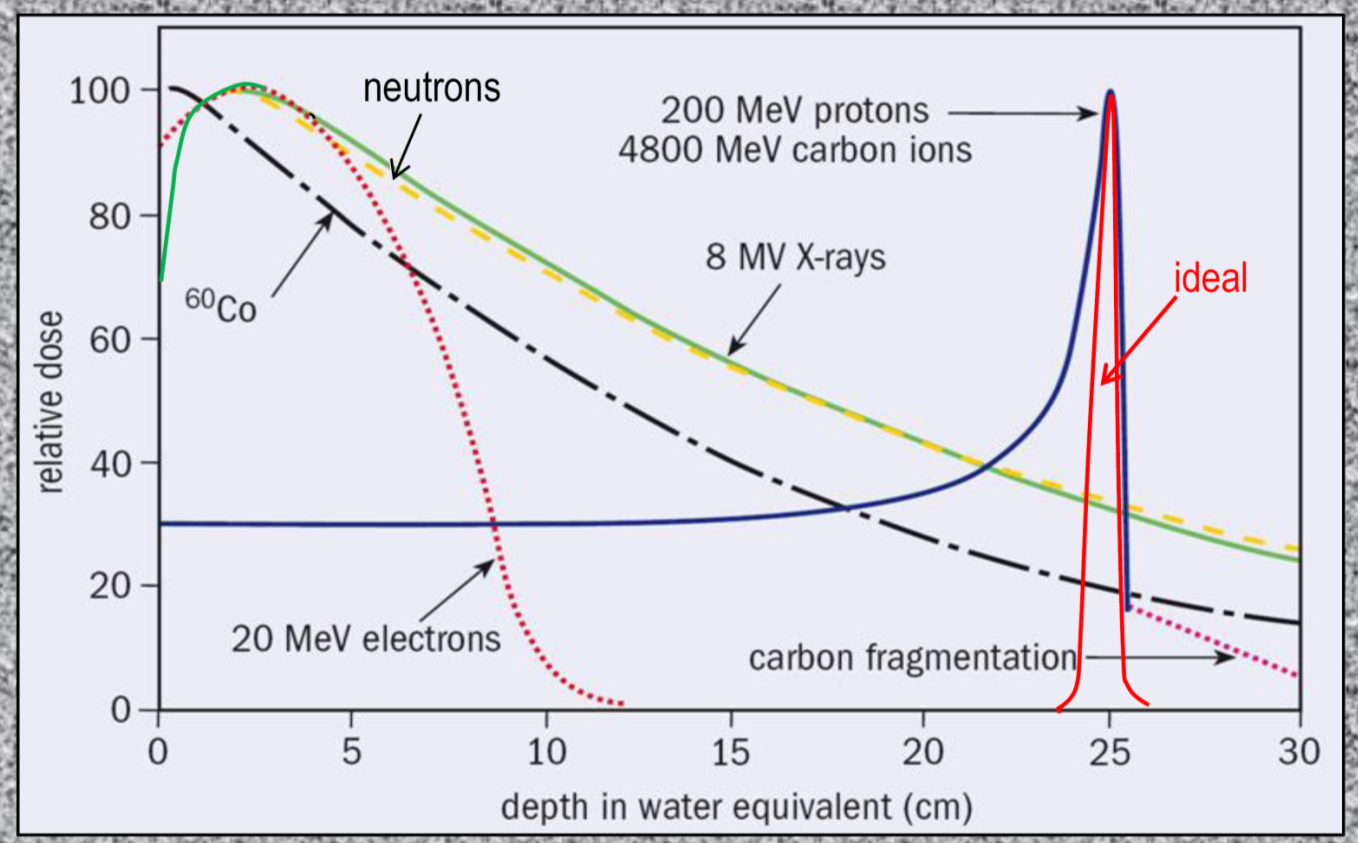
\includegraphics[width=.95\textwidth, height=0.8\textheight, keepaspectratio]{bragg_peak.png}
\end{center}
}


\subsection{Particle accelerators: how?}

\frame{
\frametitle{A simple synchrotron}
%\framesubtitle {Hadron therapy}
\begin{center}
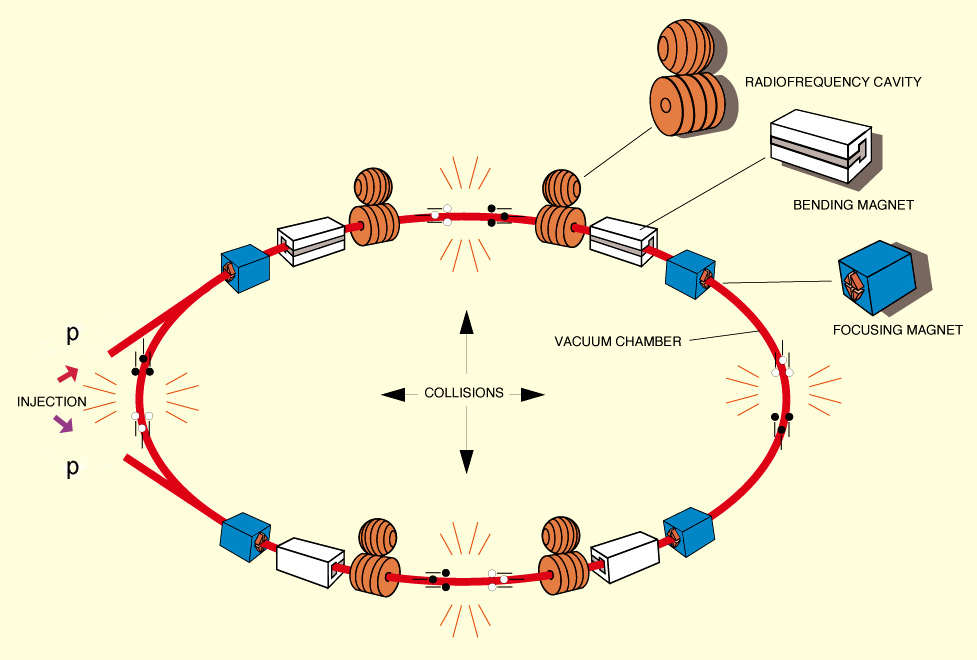
\includegraphics[width=.95\textwidth, height=0.8\textheight, keepaspectratio]{synchrotron.jpg}
\end{center}
}

\frame{
\frametitle{LEP superconducting cavity}
%\framesubtitle {Hadron therapy}
\begin{center}
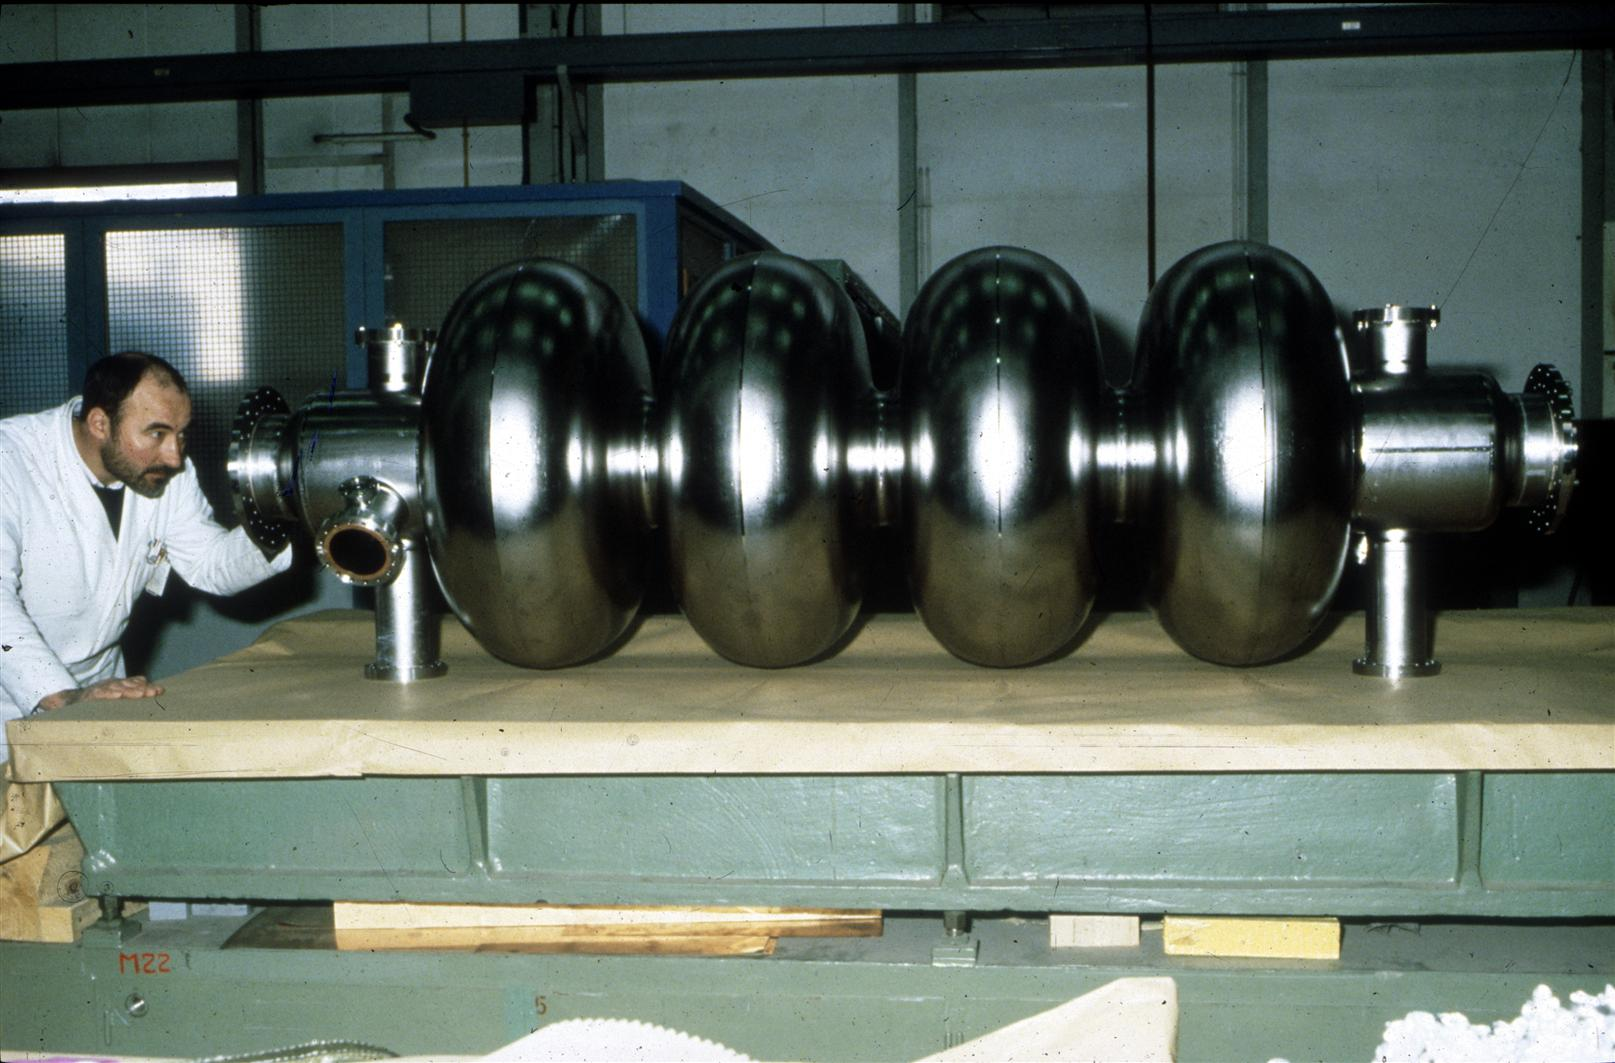
\includegraphics[width=.95\textwidth, height=0.8\textheight, keepaspectratio]{lep_cavity.jpg}
\end{center}
}

\frame{
\frametitle{CLIC cavity}
%\framesubtitle {Hadron therapy}
\begin{center}
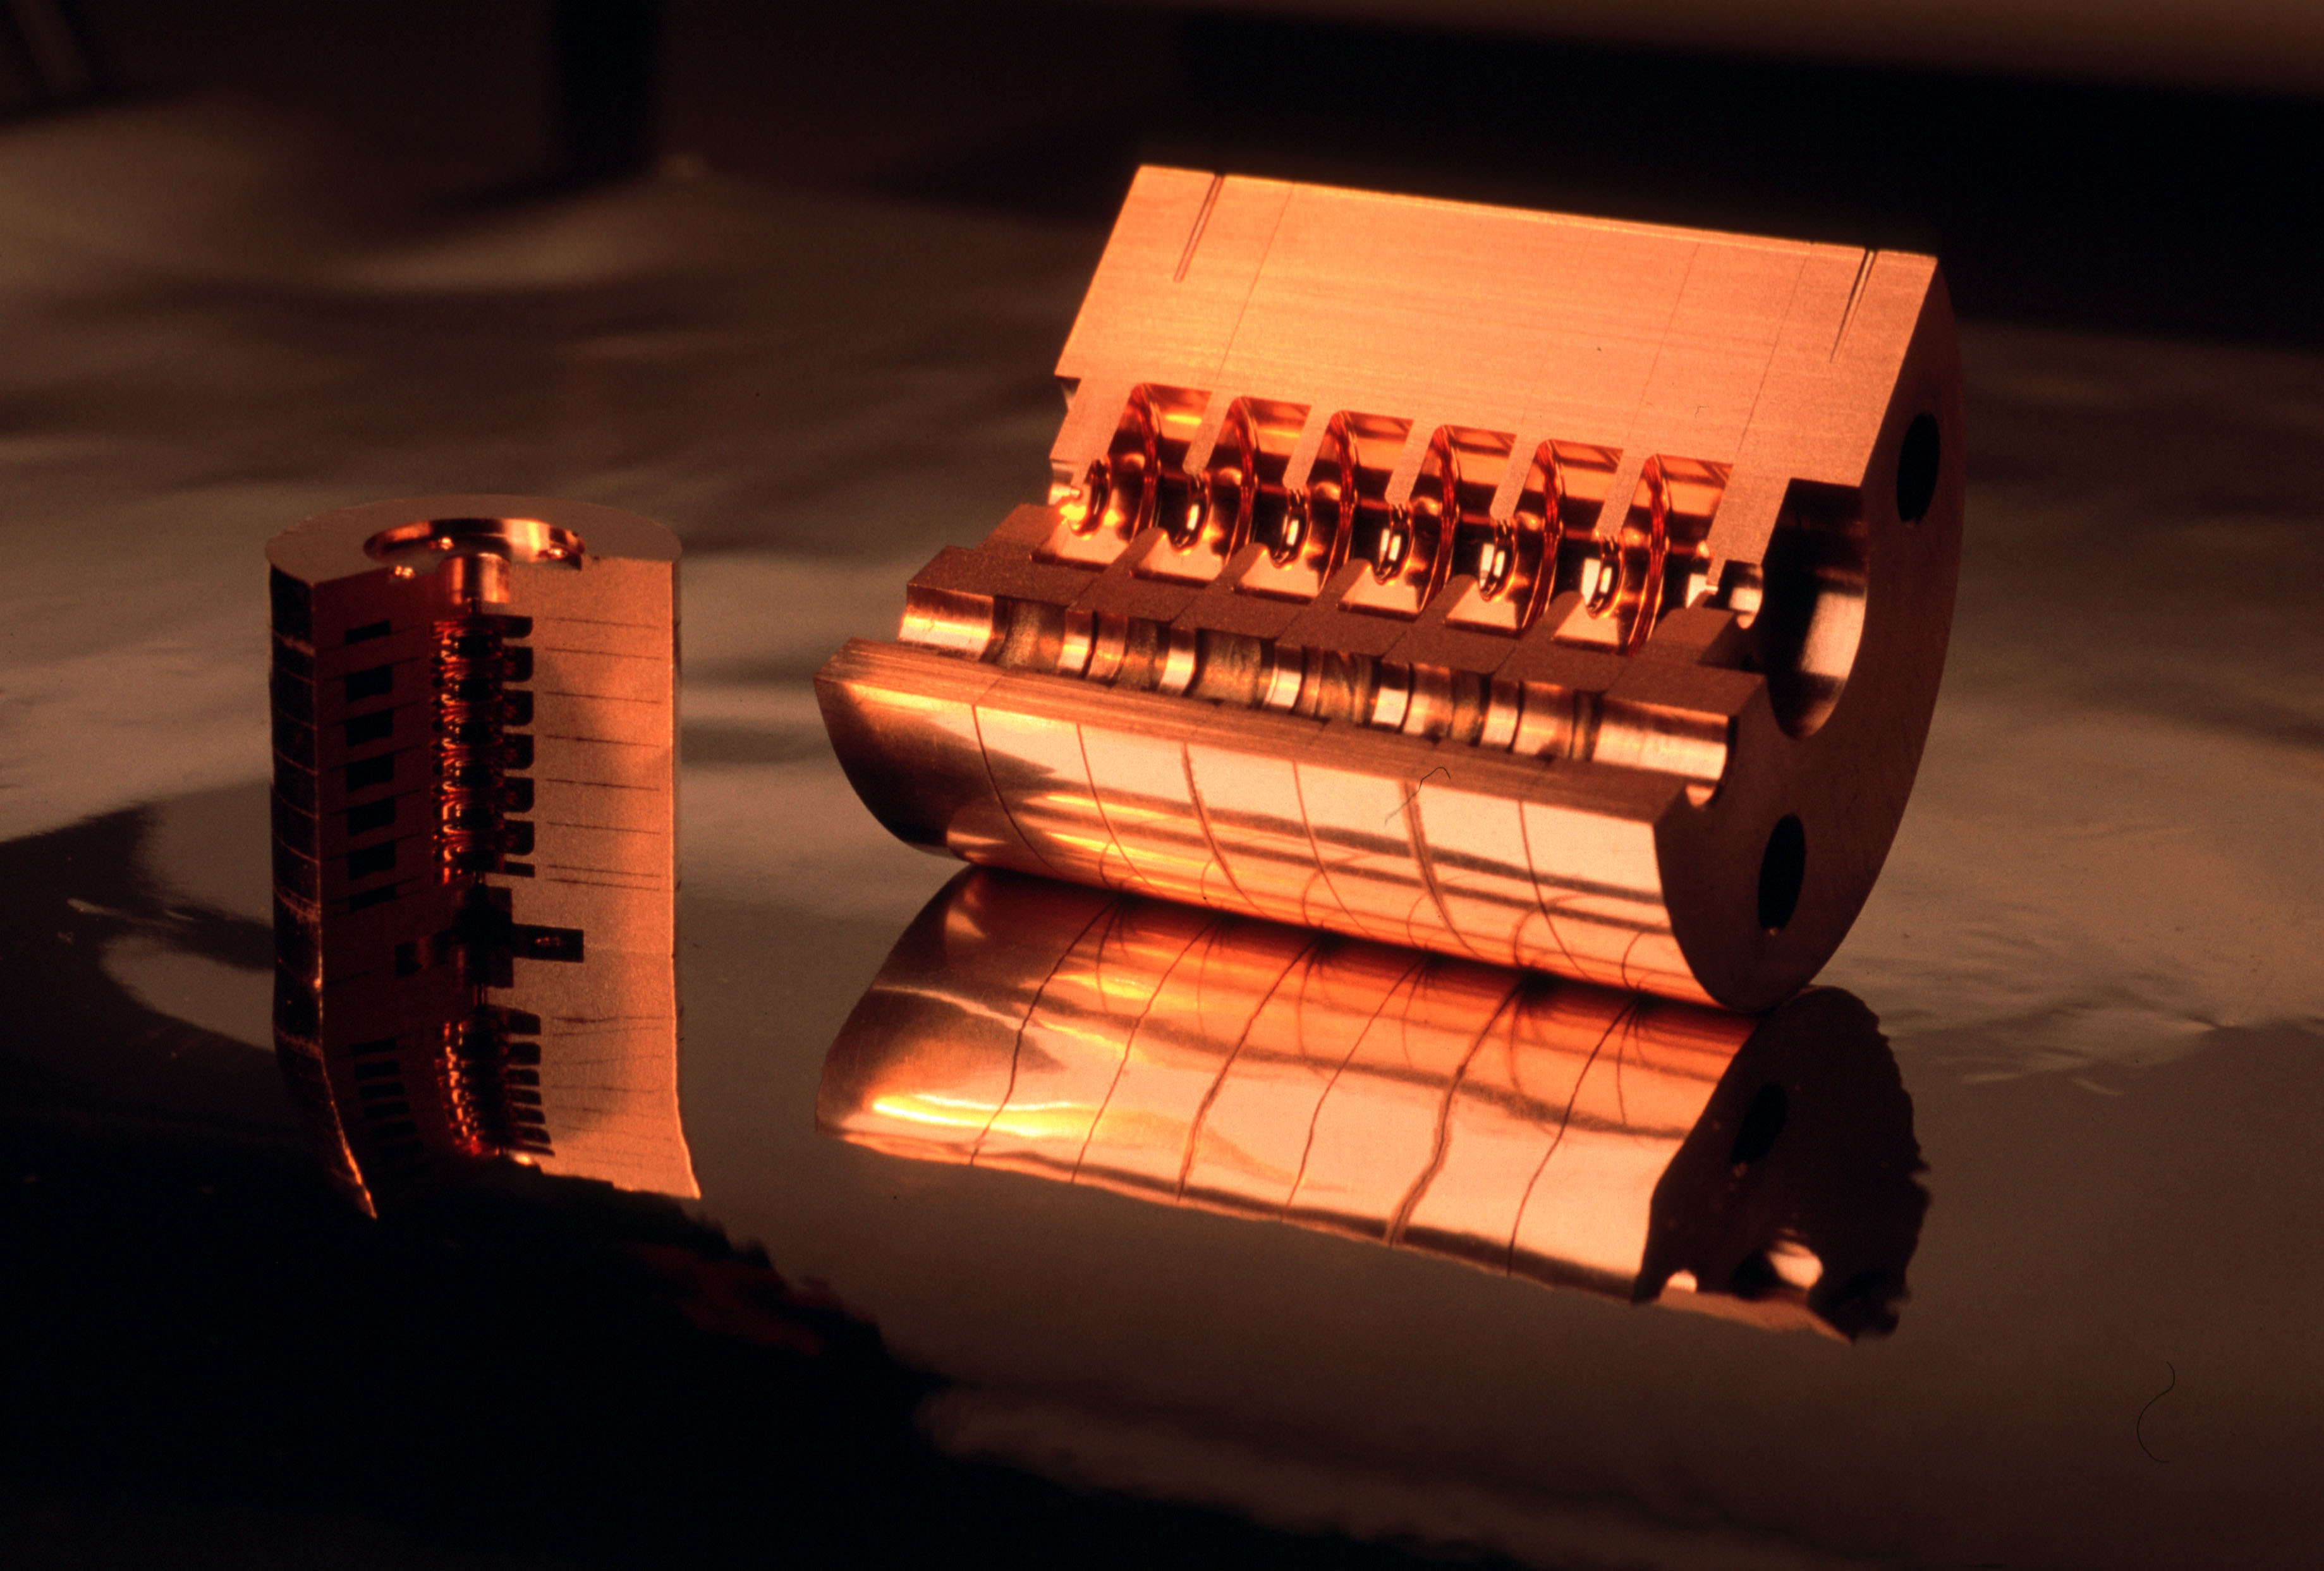
\includegraphics[width=.95\textwidth, height=0.8\textheight, keepaspectratio]{clic_cavity.jpg}
\end{center}
}

\frame{
\frametitle{Drift Tube Linac (DTL)}
%\framesubtitle {Hadron therapy}
\begin{center}
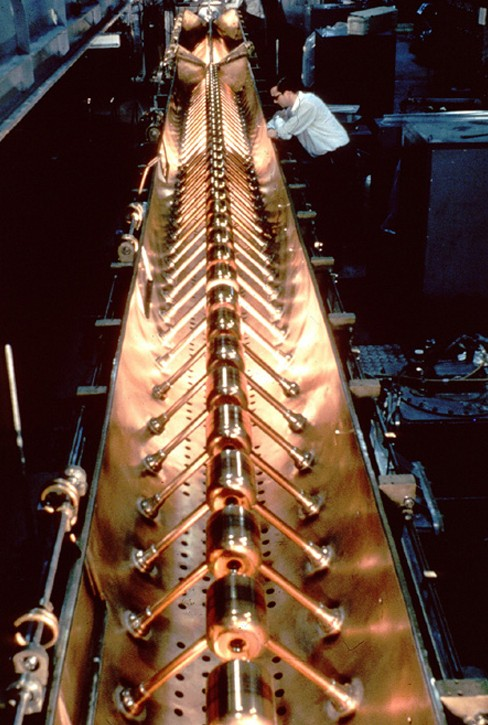
\includegraphics[width=.95\textwidth, height=0.8\textheight, keepaspectratio]{drift_tube_linac.jpg}
\end{center}
}

\frame{
\frametitle{A simple dipole electromagnet}
%\framesubtitle {Hadron therapy}
\begin{center}
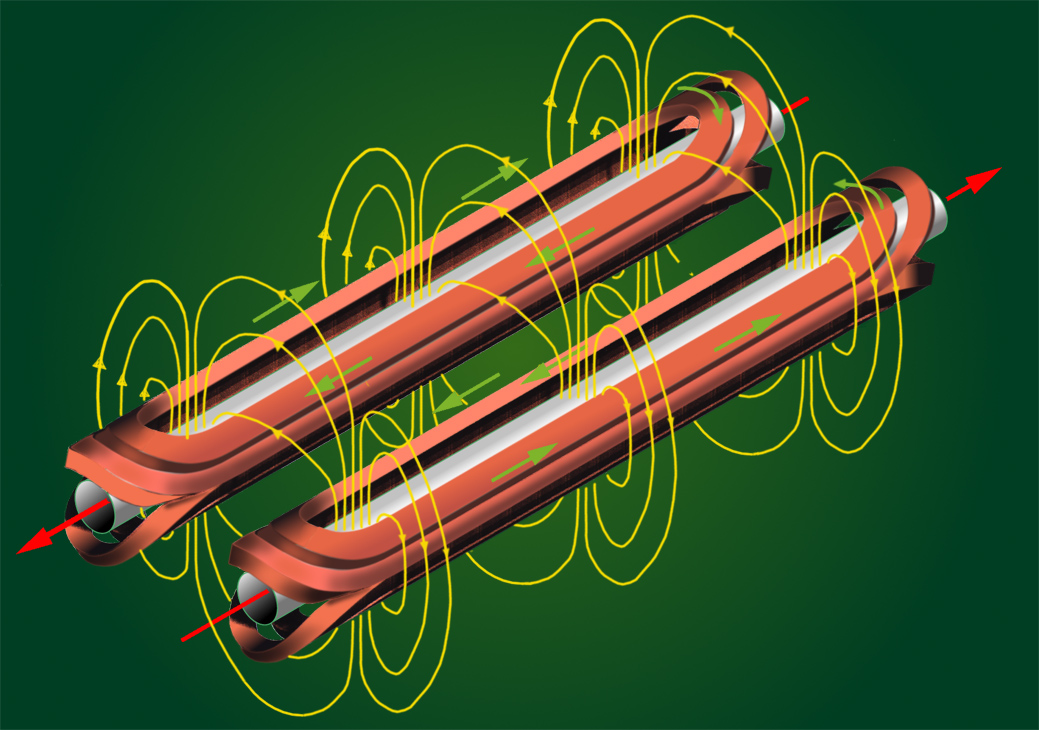
\includegraphics[width=.95\textwidth, height=0.8\textheight, keepaspectratio]{dipole_magnet.jpg}
\end{center}
}

\frame{
\frametitle{LHC cryodipole}
%\framesubtitle {Hadron therapy}
\begin{center}
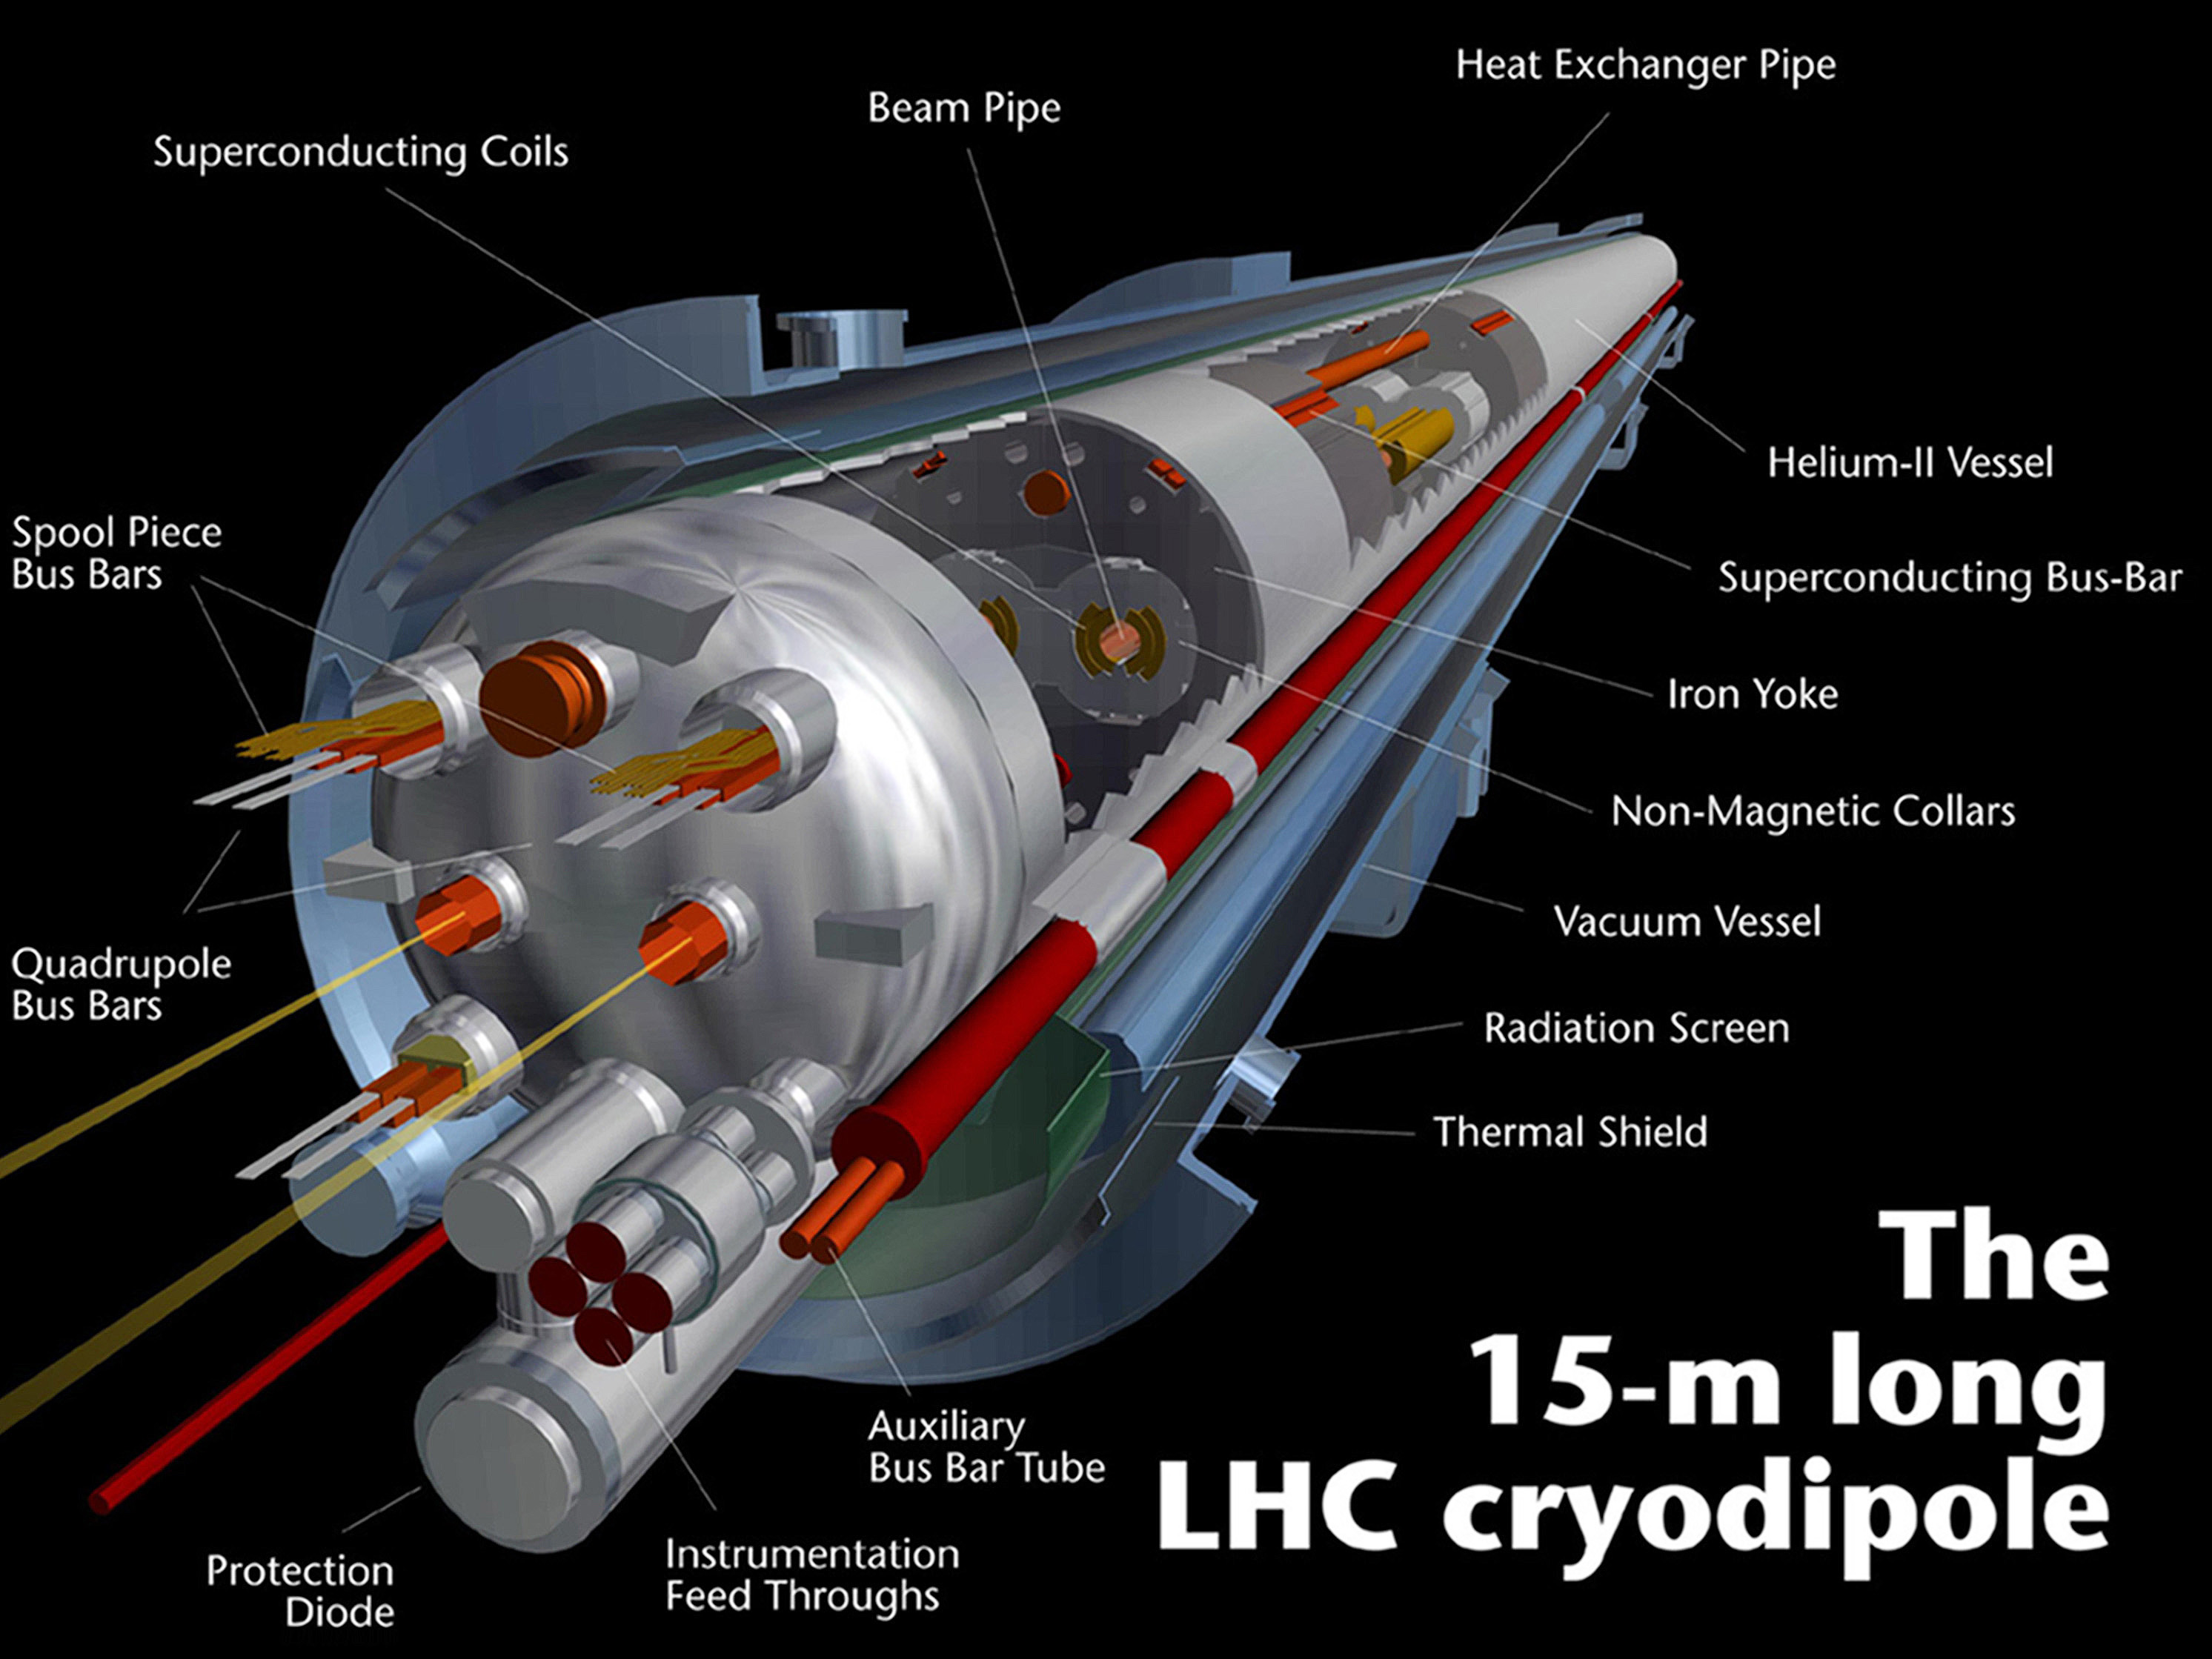
\includegraphics[width=.95\textwidth, height=0.8\textheight, keepaspectratio]{lhc_dipole.jpg}
\end{center}
}

\frame{
\frametitle{ATLAS on paper}
%\framesubtitle {Hadron therapy}
\begin{center}
\includegraphics[width=.95\textwidth, height=0.8\textheight, keepaspectratio]{atlas_diagram.jpg}
\end{center}
}

\frame{
\frametitle{ATLAS in reality}
%\framesubtitle {Hadron therapy}
\begin{center}
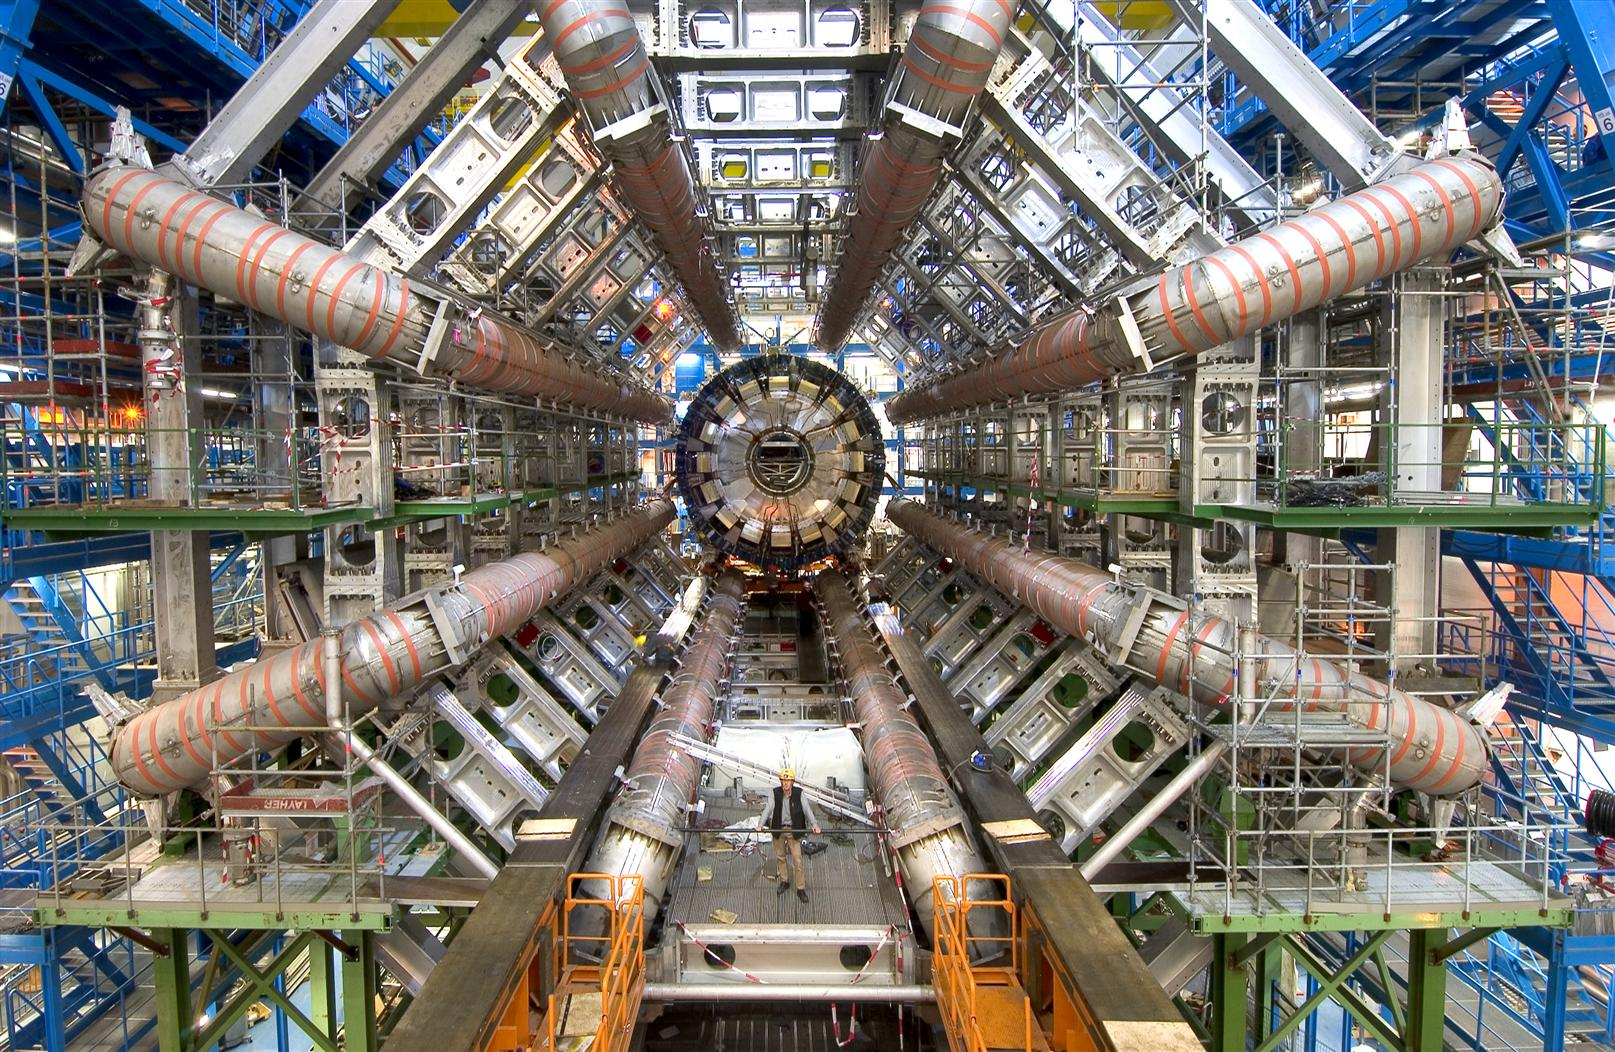
\includegraphics[width=.95\textwidth, height=0.8\textheight, keepaspectratio]{atlas.jpg}
\end{center}
}

\frame{
\frametitle{ATLAS event example}
%\framesubtitle {Hadron therapy}
\begin{center}
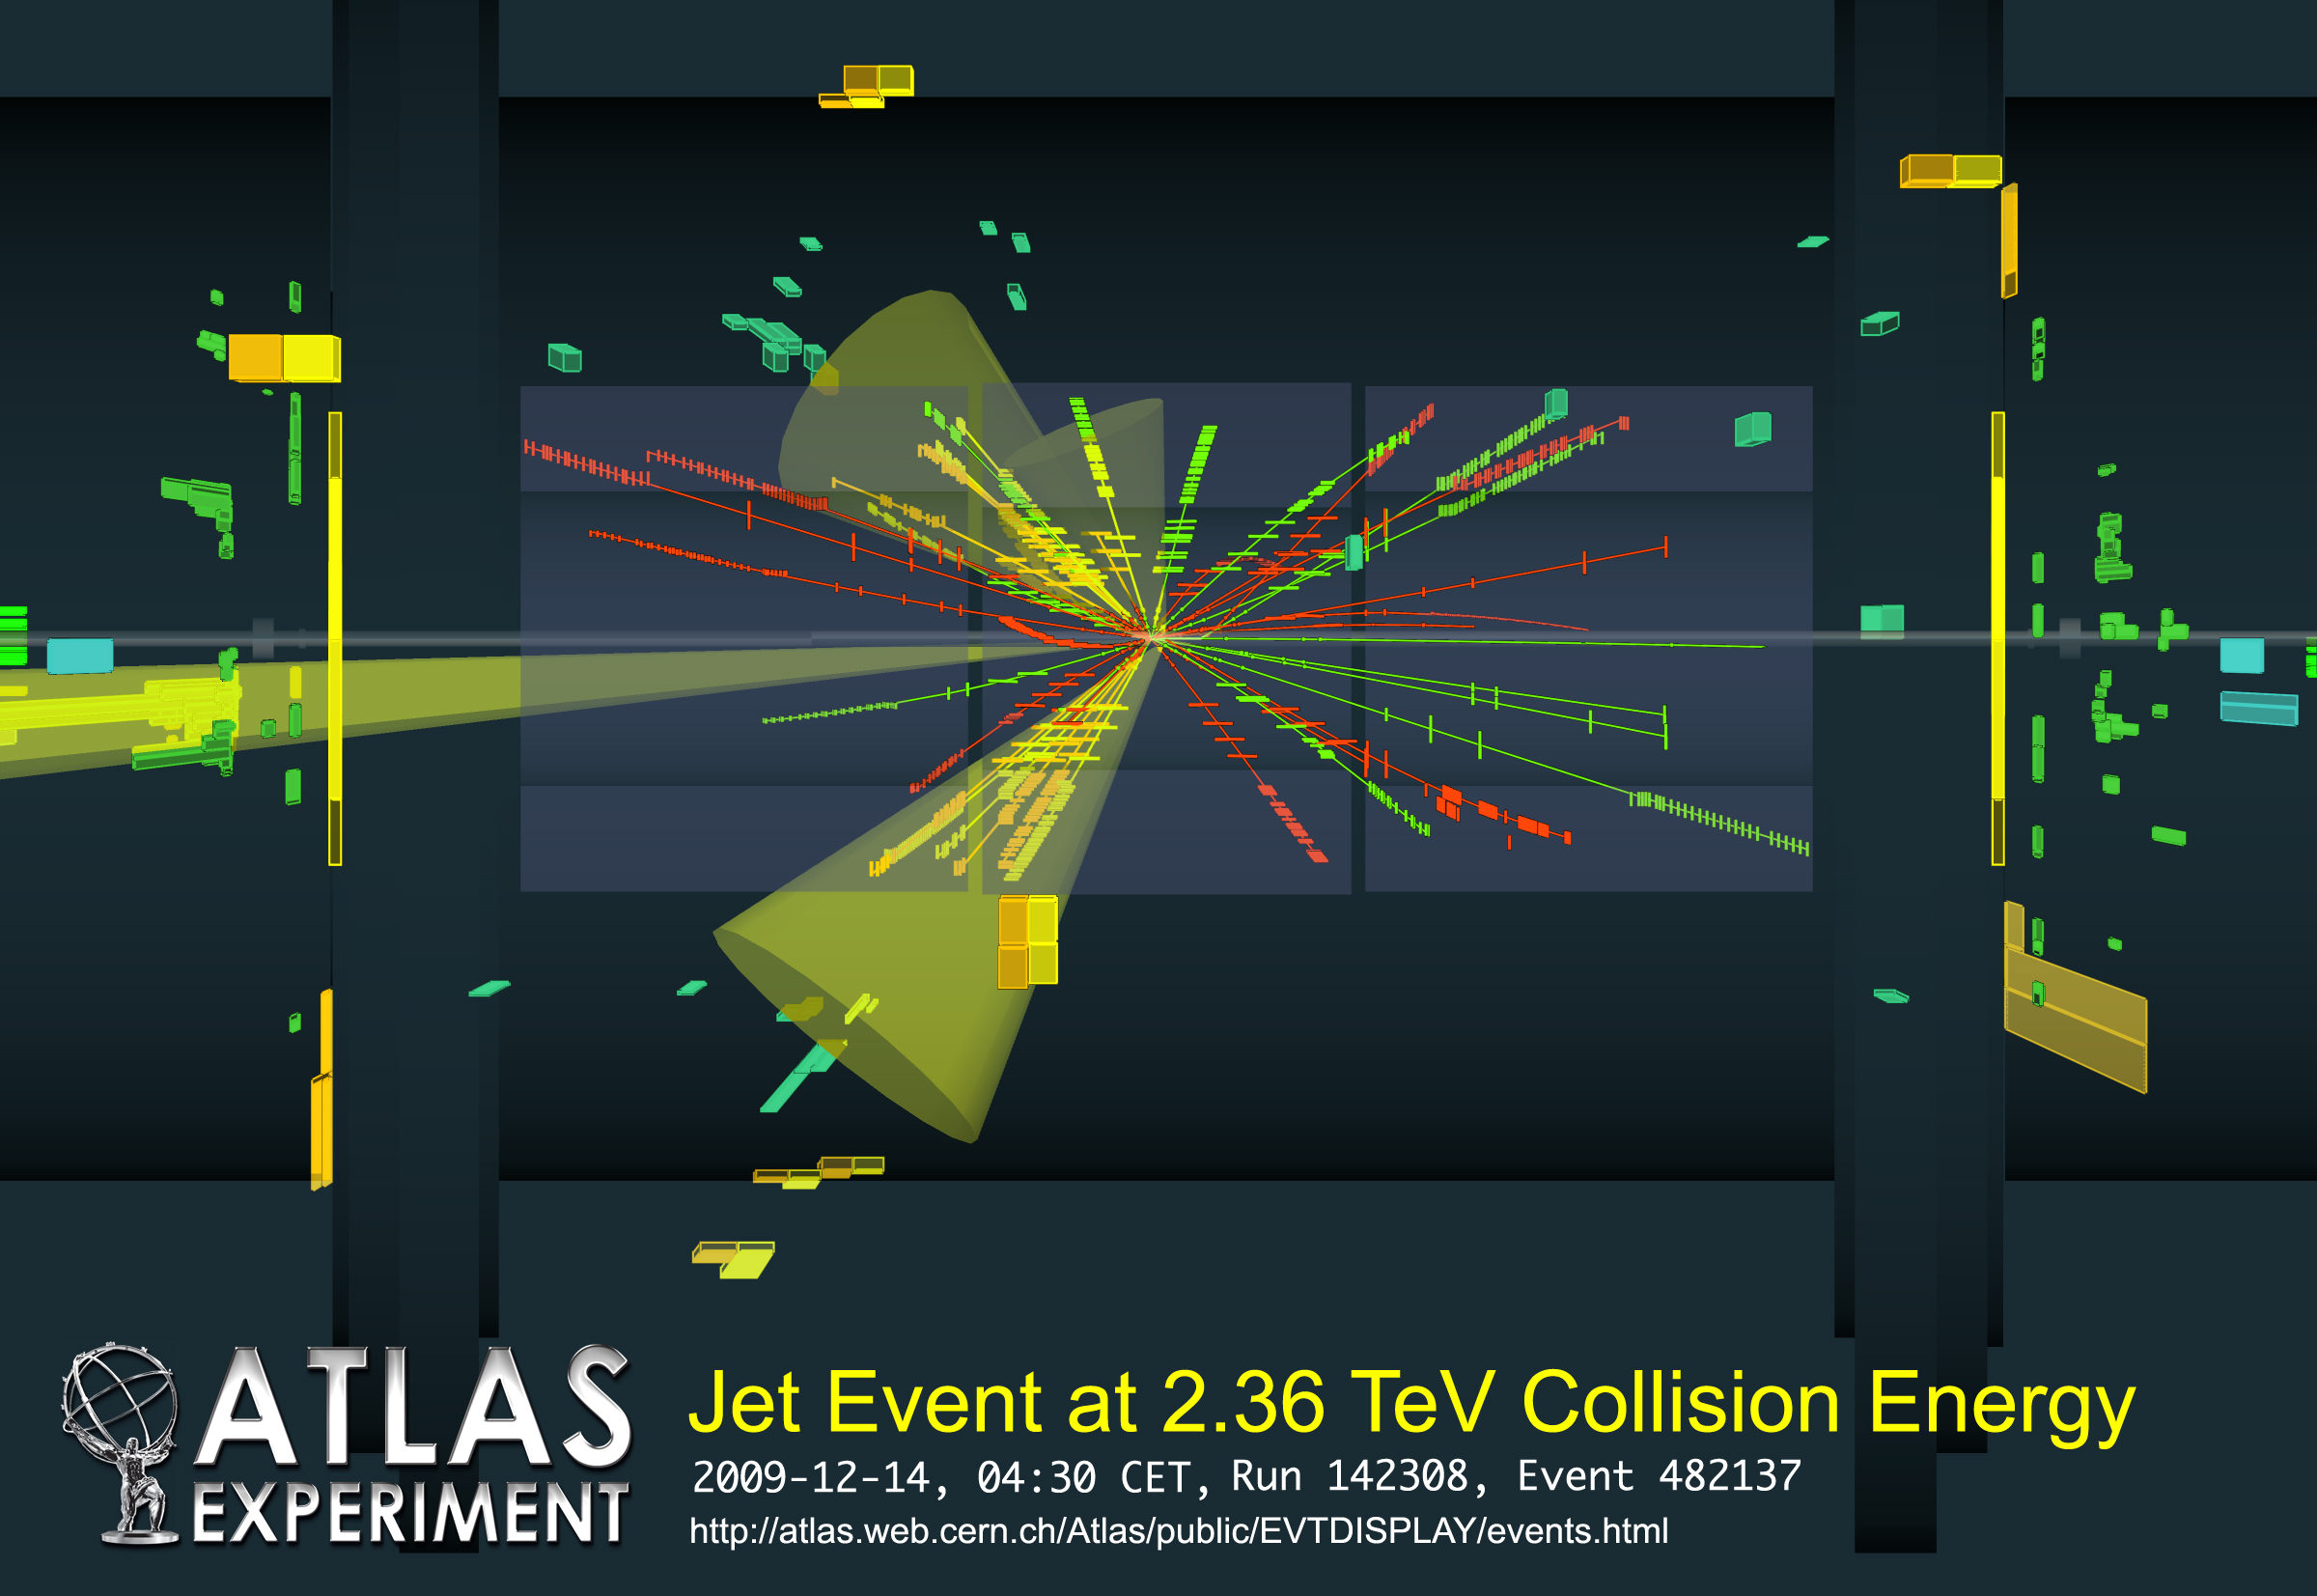
\includegraphics[width=.95\textwidth, height=0.8\textheight, keepaspectratio]{atlas_event.jpg}
\end{center}
}

\frame{
\frametitle{Free Electron Laser}
%\framesubtitle {Hadron therapy}
\begin{center}
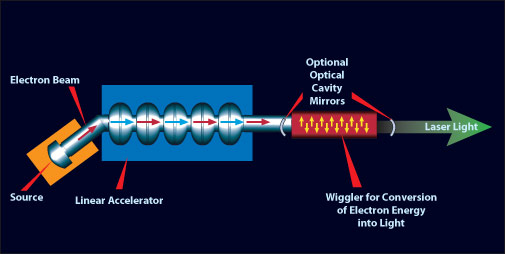
\includegraphics[width=.95\textwidth, height=0.8\textheight, keepaspectratio]{fel.jpg}
\end{center}
}

\section{Overview of Controls Hardware}

\begin{frame}{CERN Beams Controls group}
\begin{block}{Responsible for}
  \begin{itemize}
  \item 
    Controls infrastructure for all CERN accelerators, transfer lines and experimental areas
  \item 
   General services such as synchronization and analog signal acquisition/display
  \item 
    Specification, design, procurement, integration, installation, commissioning and operation
  \end{itemize}
\end{block}

\begin{block}{Supports}
  \begin{itemize}
  \item beam instrumentation, cryogenics, power converters etc.
  \end{itemize}
\end{block}

\end{frame}


\begin{frame}{Beams Controls standard kit}

\begin{block}{Hardware kit}
  \begin{itemize}
      \item  analog and digital I/O
      \item level converters, repeaters
      \item serial links, timing modules
    \end{itemize}
\end{block}


\begin{block}{Software}
  \begin{itemize}
  \item Linux device drivers, C/C++ libraries, test programs
  \end{itemize}
\end{block}

\end{frame}

\section{Standards for New Designs}

\subsection{Bus standards}

\begin{frame}{Bus standards for new designs}
	\begin{block}{Two bus standards}
	  \begin{itemize}
		\item VME64x
		      \begin{itemize}
			\item 6U, large front-panel space, may use rear transition module
		       \end{itemize}
		\item PICMG 1.3
		      \begin{itemize}
			\item Industrial type PC with the processor on a plug-in board
			\item Internal buses PCI Express and PCI
		       \end{itemize}
	   \end{itemize}
	\end{block}

	\begin{block}{Need for a mezzanine approach}
	  \begin{itemize}
		\item Functions (e.g. ADC, TDC) are needed for both buses
		\item Would need twice as many designs, more if additional standards are needed (PXIe, xTCA)
%		\item Using a carrier with the I/O functionality on a mezzanine reduces design work
	   \end{itemize}
	\end{block}
\end{frame}

\begin{frame}{Carriers and mezzanines}
 \begin{columns}
 \begin{column}{5cm}
  \begin{center}
   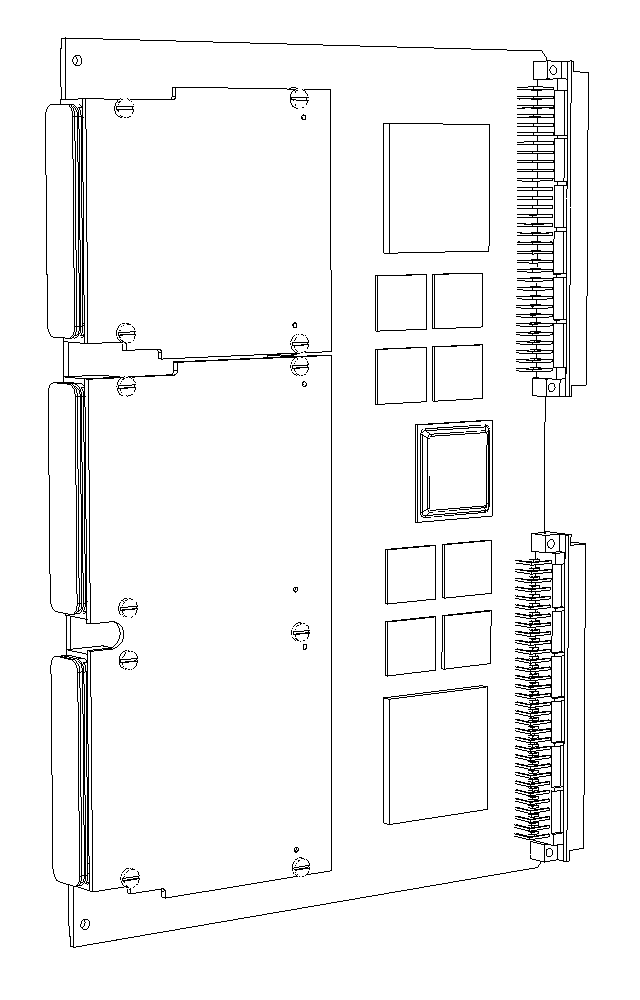
\includegraphics[width=3.5cm]{carrier.png}%
  \end{center}
 \end{column}
 \begin{column}{5cm}
  \begin{center}
   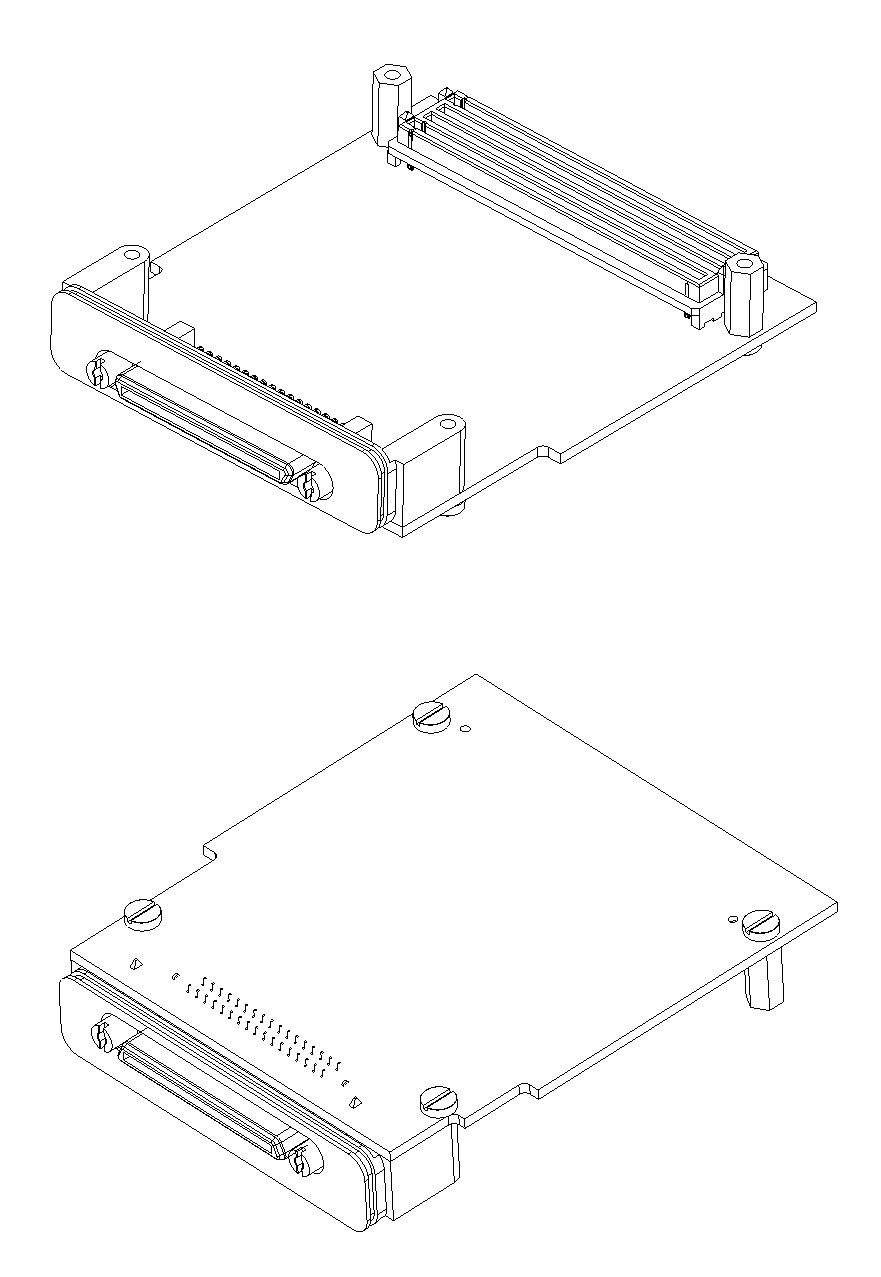
\includegraphics[width=3.5cm]{single_width1.png}%
  \end{center}
 \end{column}
 \end{columns}
 Courtesy of VITA: http://www.vita.com/fmc.html
\end{frame}

\subsection{FPGA Mezzanine Card (FMC)}
%=========================

\begin{frame}{Advantages of the carrier/mezzanine approach}
	\begin{block}{Re-use}
		- One mezzanine can be used in VME and PCIe carriers.

		- People know standards, more likely to re-use or design for it.
	\end{block}
	\begin{block}{Reactivity}
	    - Carrier: place and route a complex FPGA/Memory PCB once.

	- Mezzanine: small and easier to route cards, easy assembly.
	\end{block}
	\begin{block}{Rational split of work}
	    'Controls' can design the carrier, 'Instrumentation' an ADC mezzanine, 'RF' a DDS one, etc.
	\end{block}
\end{frame}

% IMAGES FMC
% ========

\begin{frame}{Example of a PCI Express FMC carrier (SPEC)}
 \begin{center}
   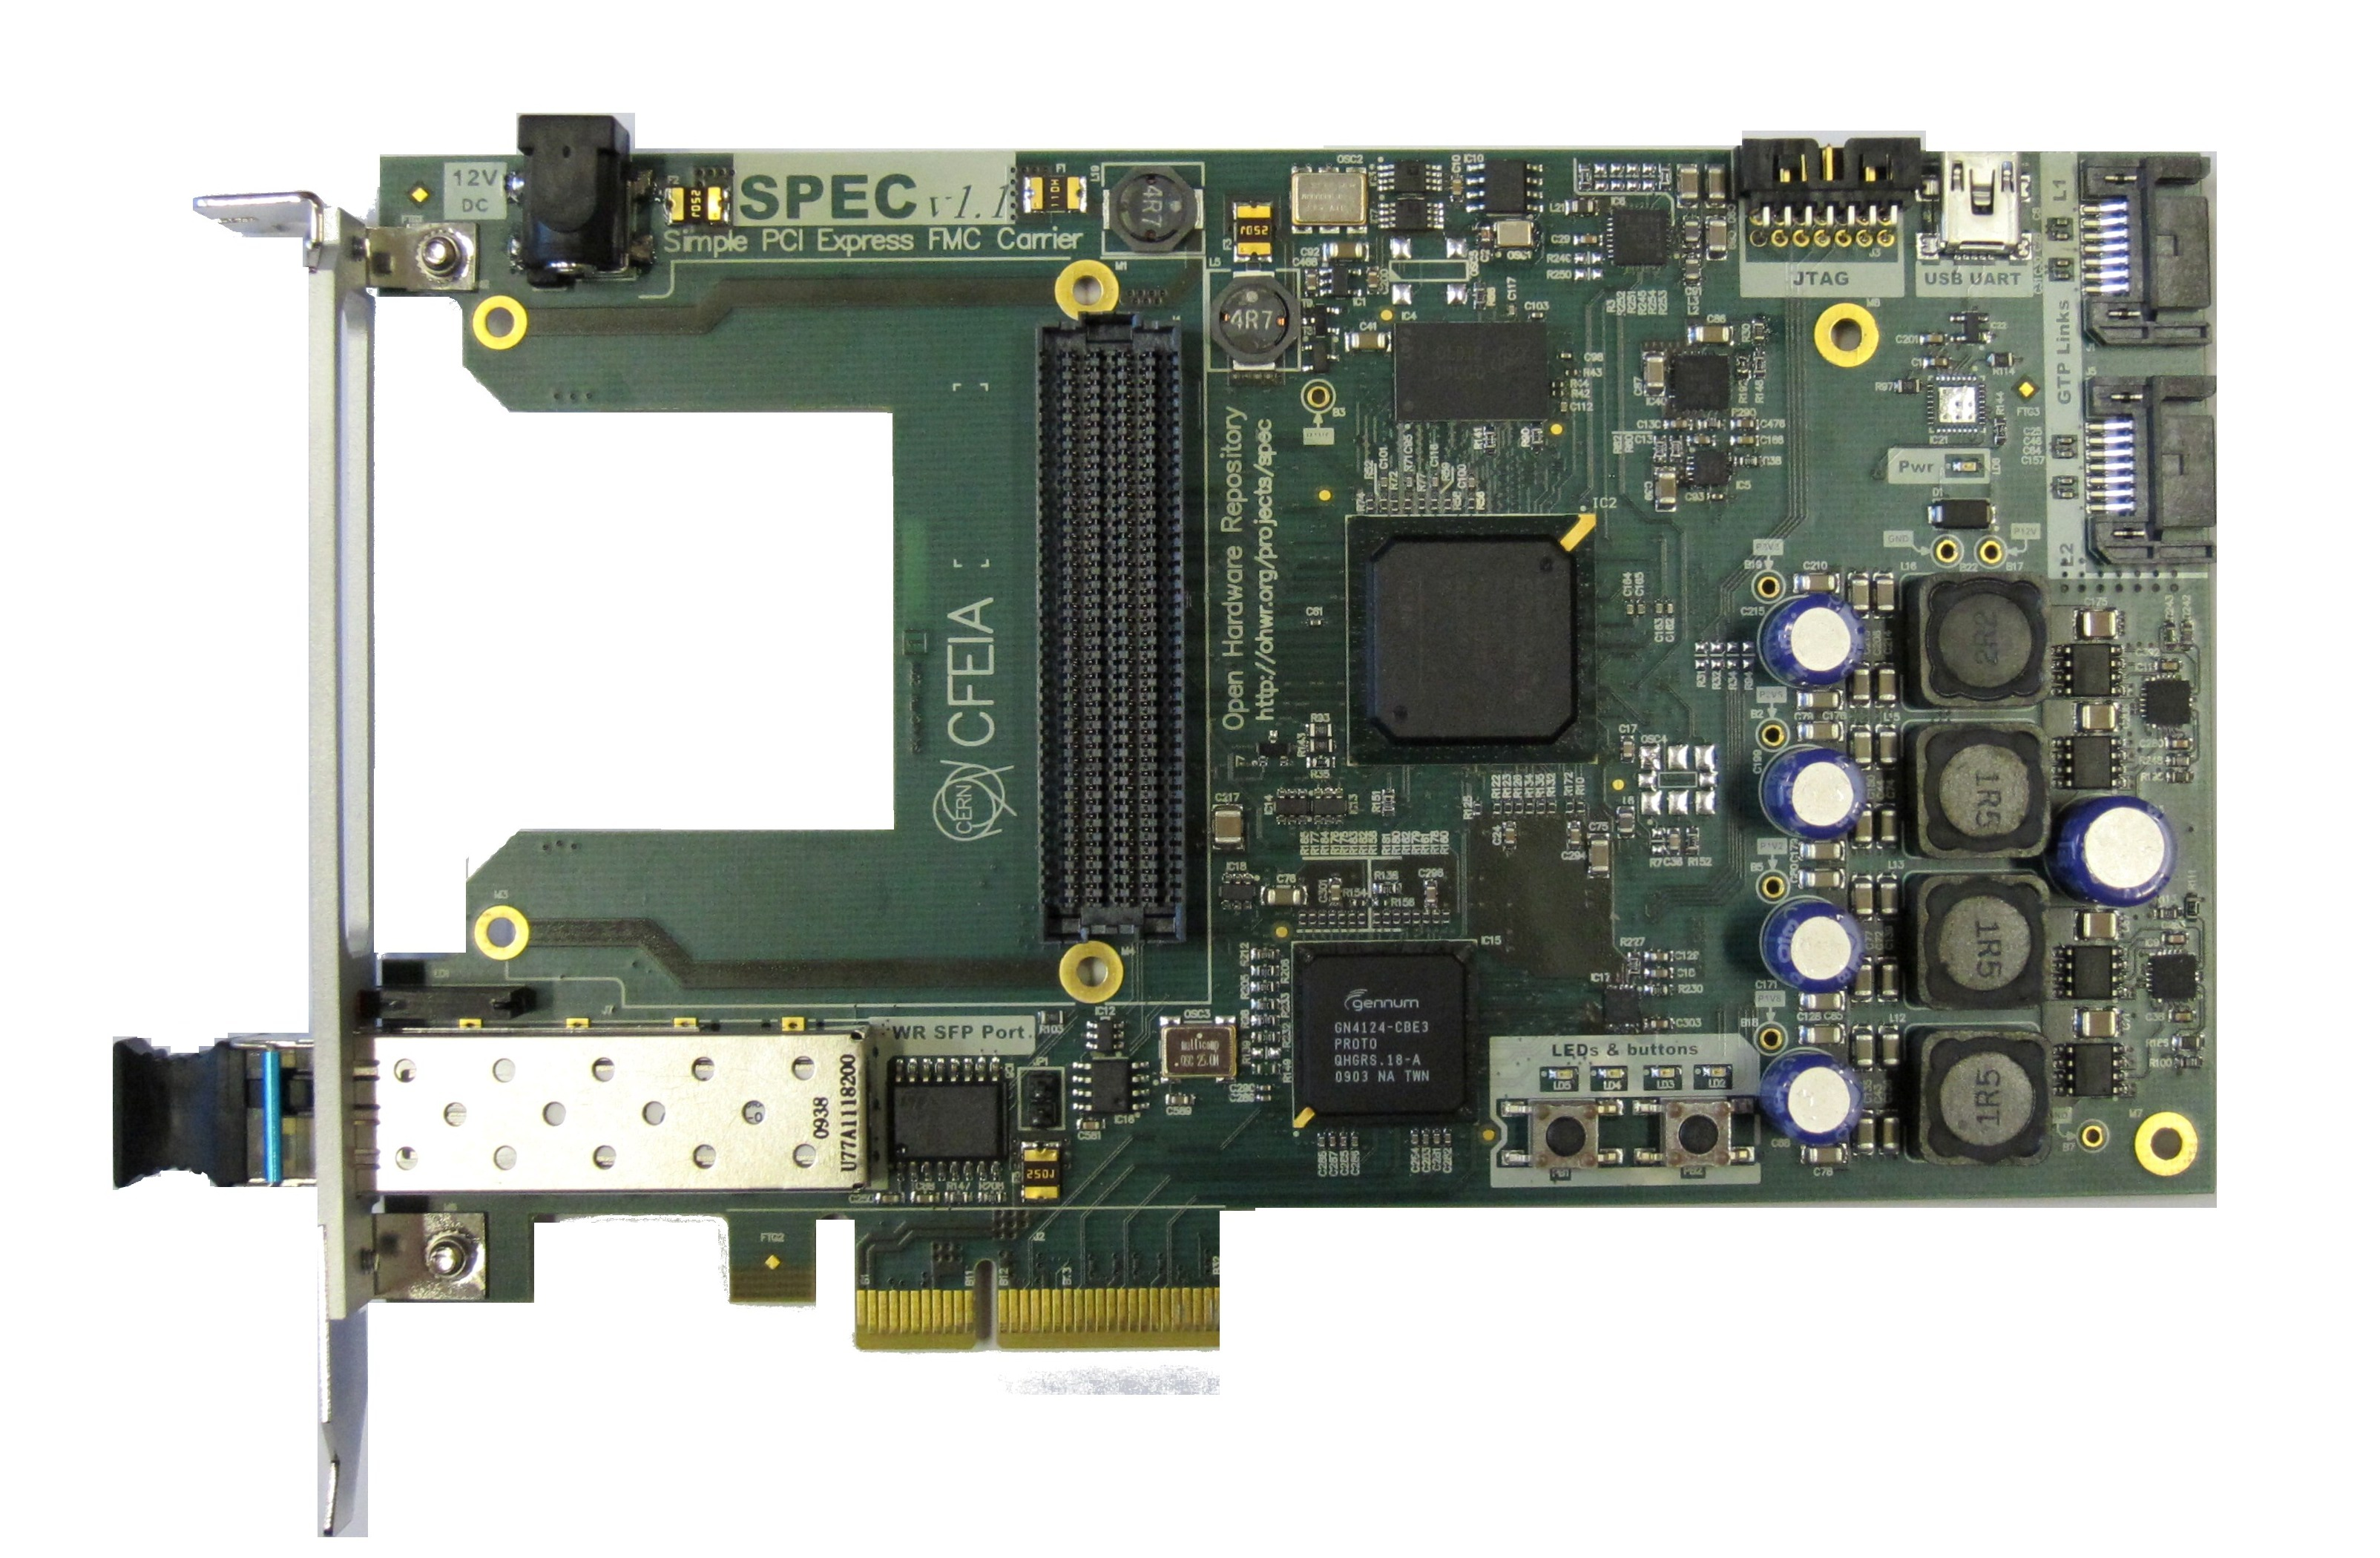
\includegraphics[height=6.8cm]{SPEC_top_high_res.jpg}
% \includegraphics[height=6cm]{../pictures/ohwr/EDA-02063-V1-0-TOP1.jpg}% ADC card
%  \includegraphics[height=6cm]{../pictures//BoardBlockDiagramv2.pdf}%
 \end{center} 
\end{frame}

\begin{frame}{Example of FMC mezzanine: 100 MSPS 14-bit 4-channel ADC}
 \begin{center}
%   \includegraphics[height=6.5cm]{../pictures/ohwr/ADC100M_EDA-02063-V1-0-TOP1.jpg}
   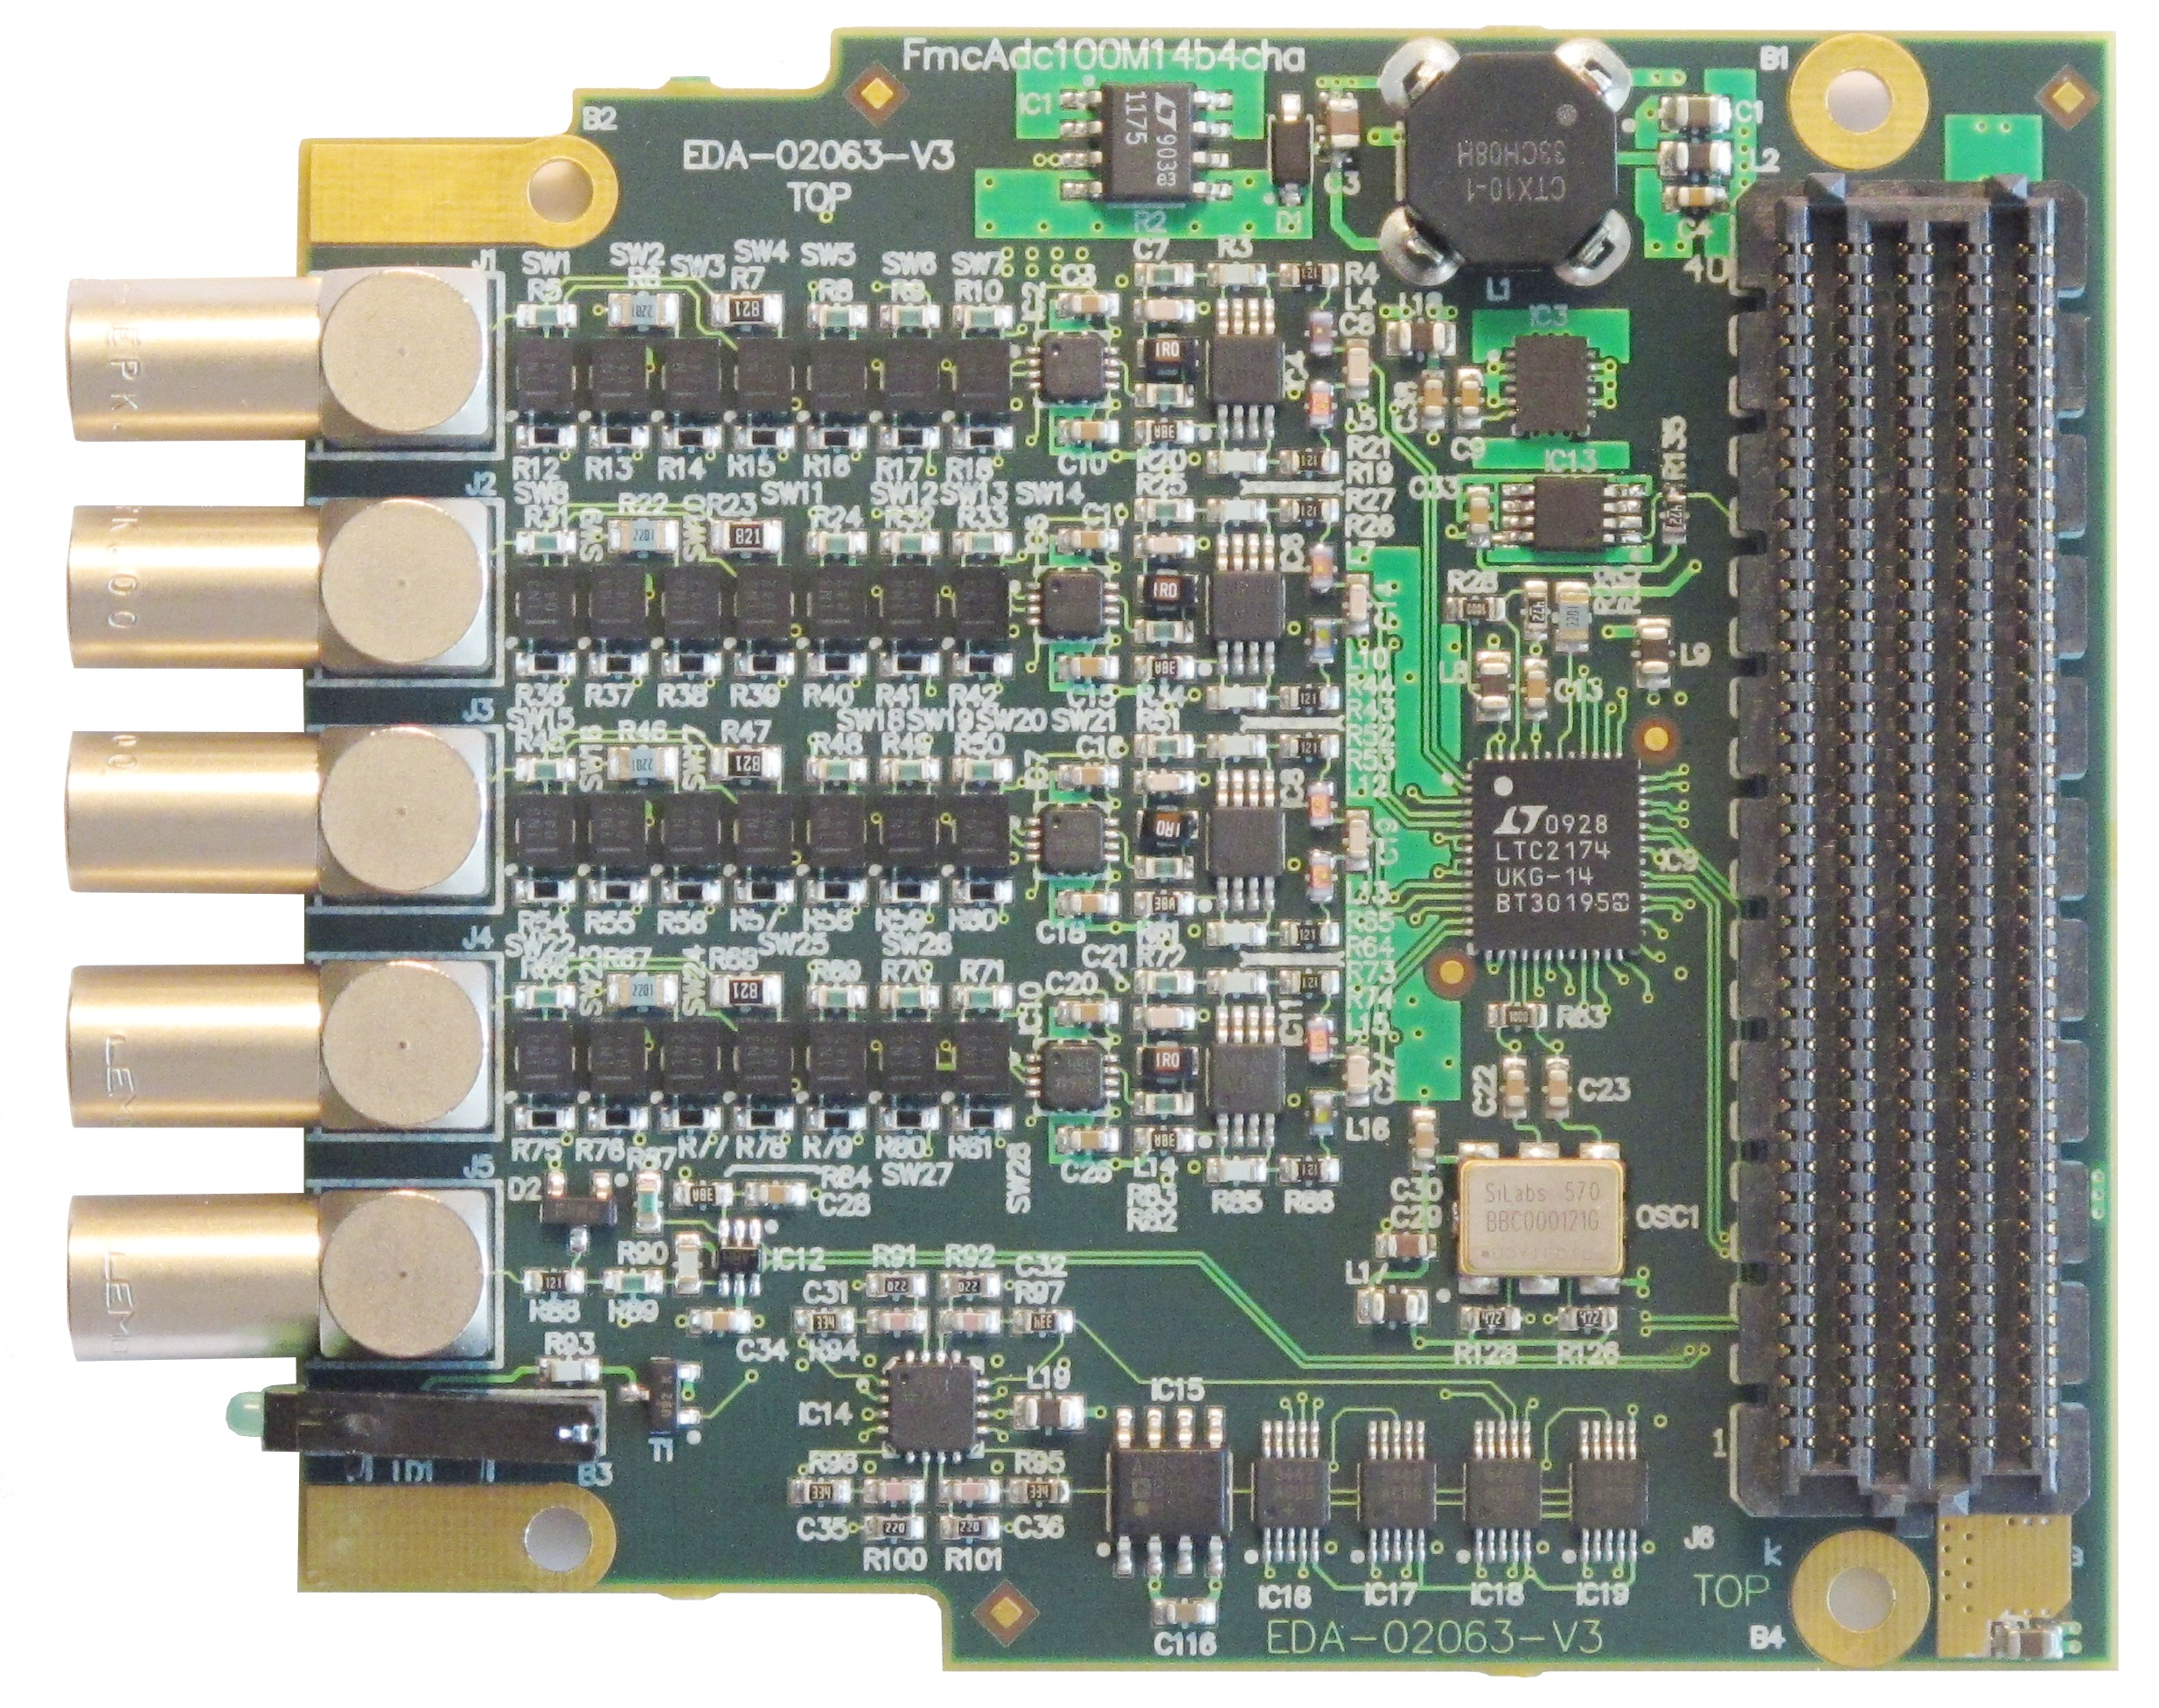
\includegraphics[height=6.5cm]{adc.jpg}
 \end{center} 
\end{frame}

\begin{frame}{VME64x FMC carrier}
 \begin{center}
%   \includegraphics[height=6.7cm]{../pictures/ohwr/VFC_picture.jpg}
   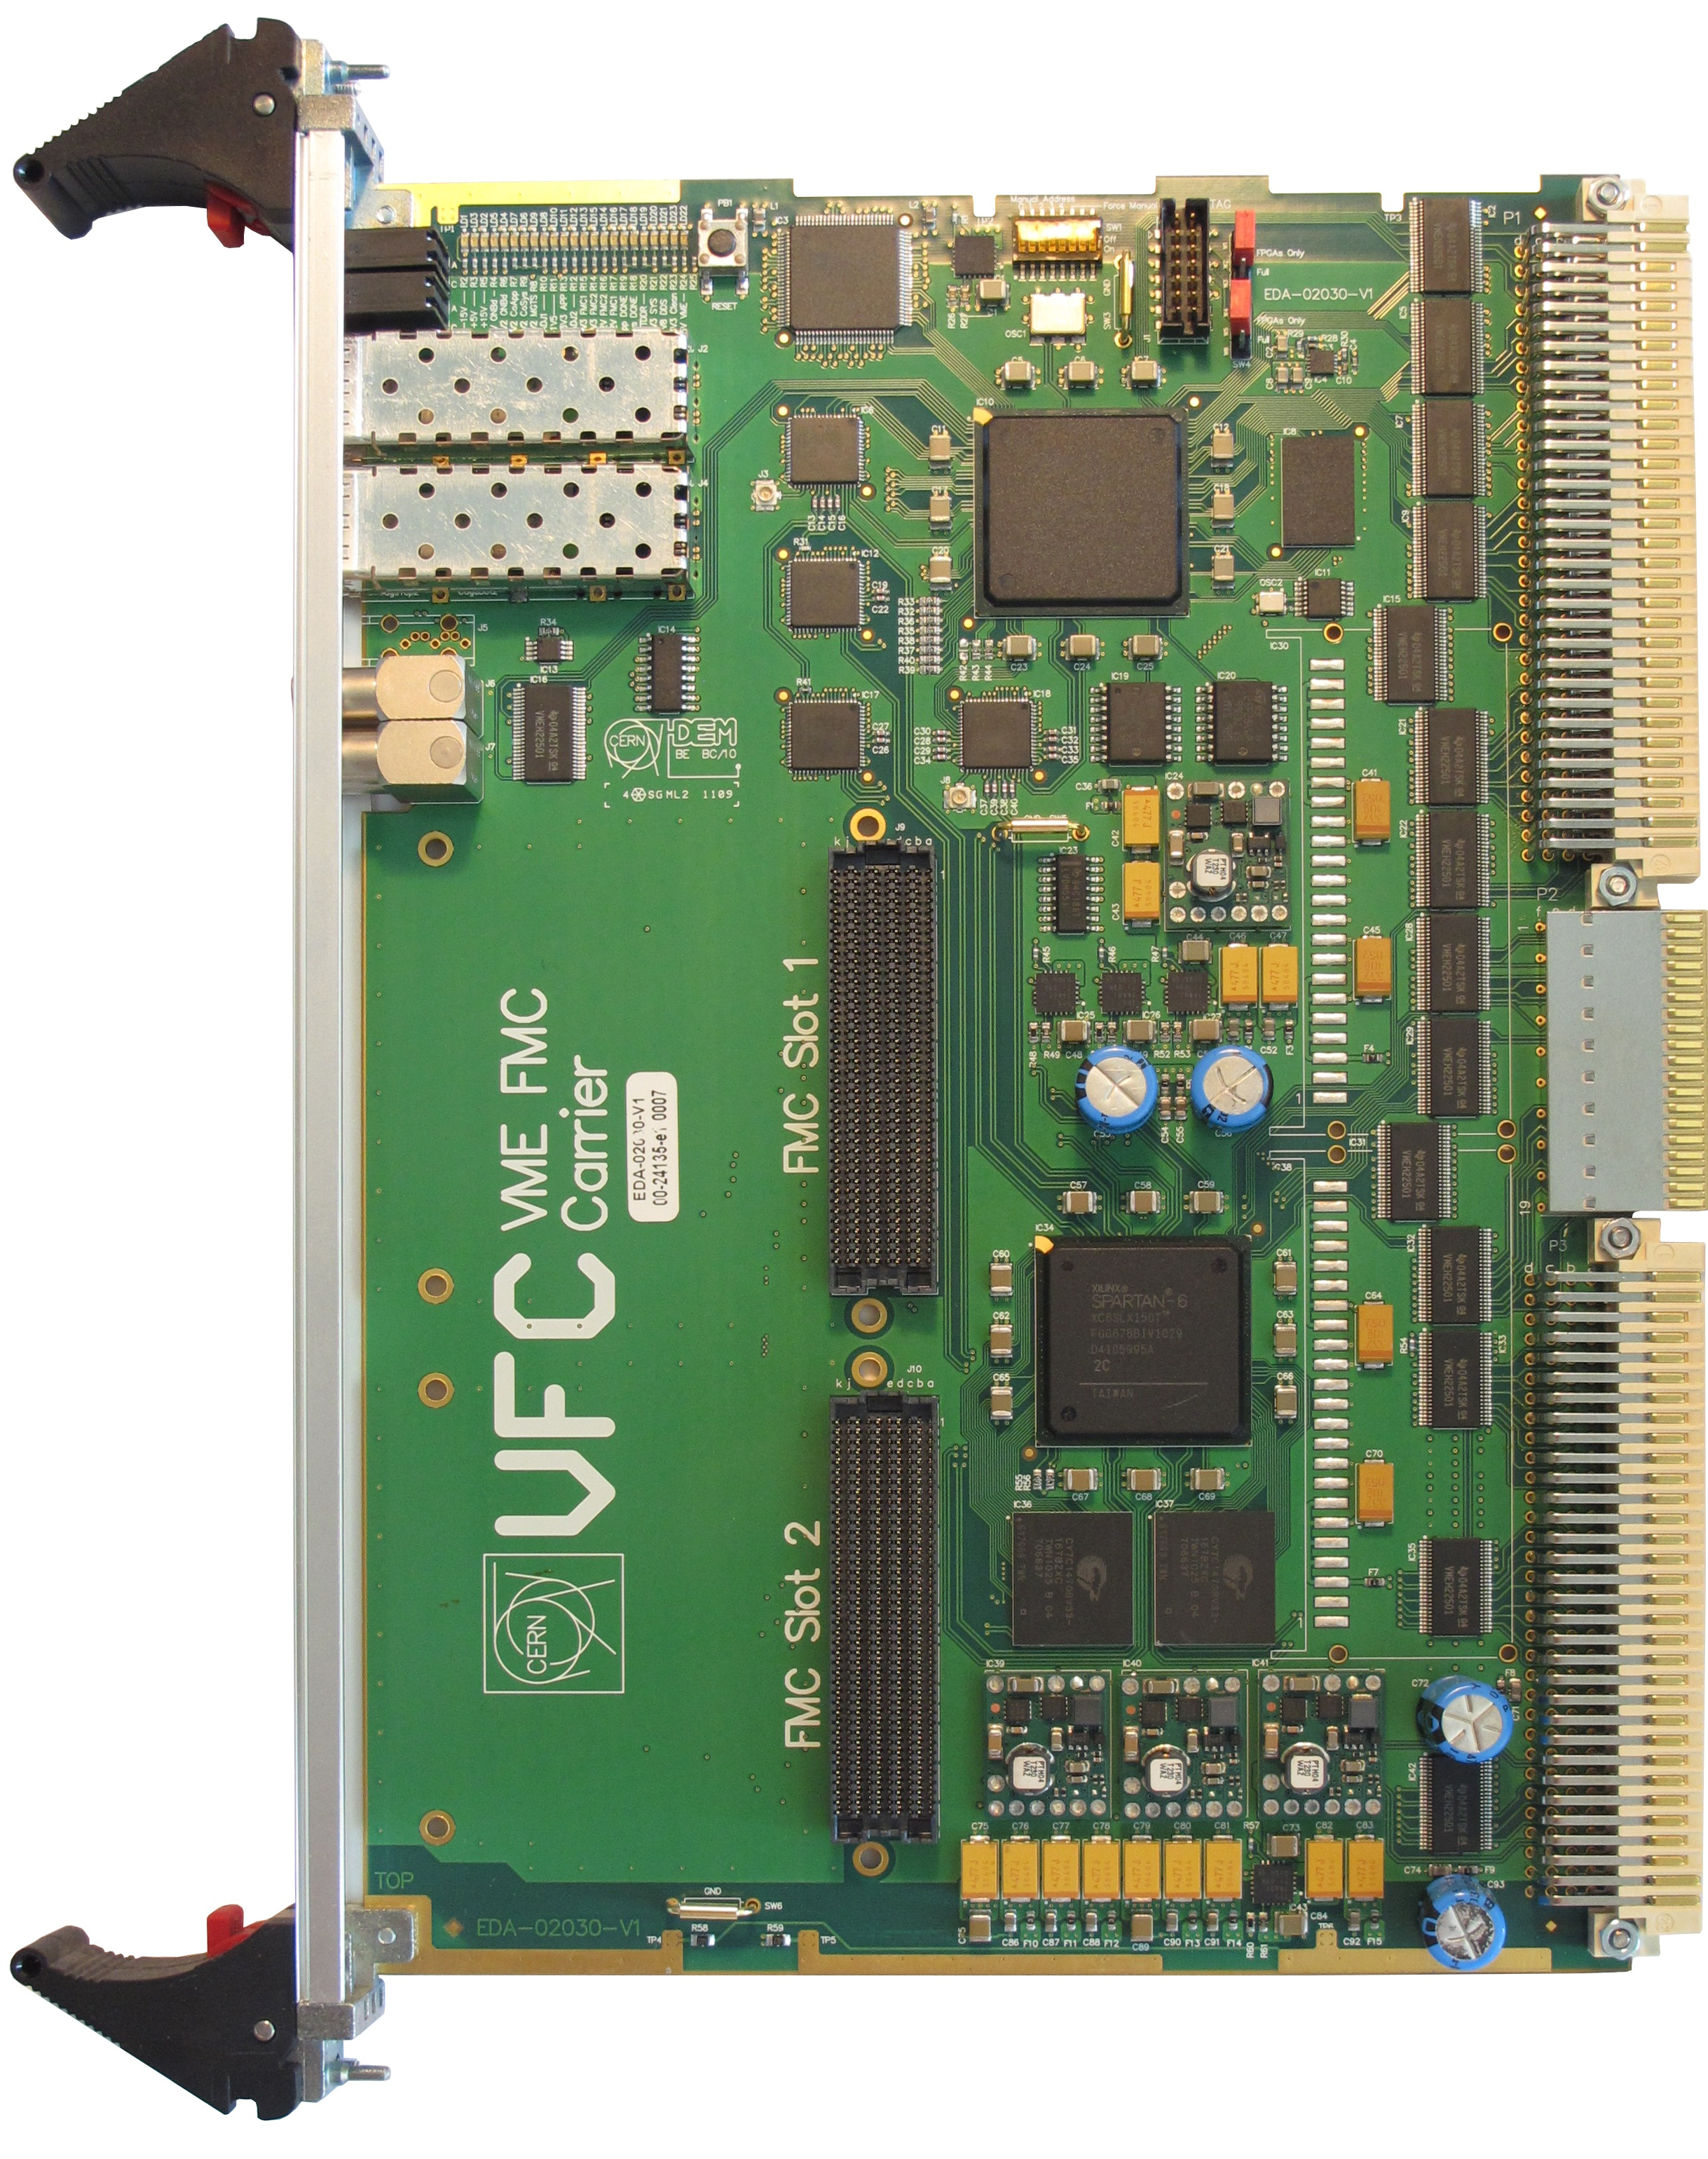
\includegraphics[height=6.9cm]{vfc.jpg}
 \end{center} 
\end{frame}

\begin{frame}{Another example of FMC mezzanine: 5-channel 1ns TDC}
 \begin{center}
   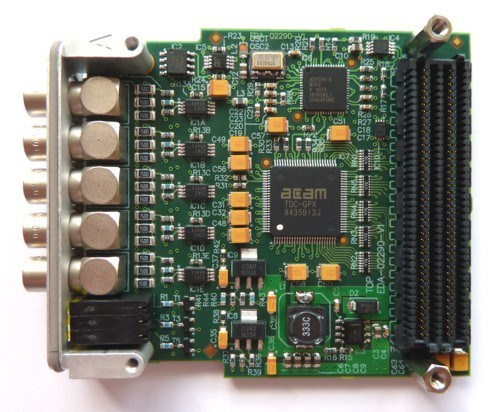
\includegraphics[height=6.5cm]{FMC_TDC_72dpi_left.jpg}
 \end{center} 
\end{frame}



\subsection{Wishbone}

\begin{frame}{Inside the FPGA: Wishbone}
 \begin{itemize}
	\item System becomes pretty complex: System-on-a-chip
	\item Build up from re-usable HDL cores
	\item Connect blocks with Wishbone bus
		\begin{itemize}
		\item open standard
		\item simple address/data bus
		\item extended with pipelined mode
		\item many cores already available
		\end{itemize}
	\item We developed a design infrastructure
		\begin{itemize}
		\item \textcolor{red}{WBGen}: scripts to automatically generate Wishbone slave
                  HDL and documentation
		\item \textcolor{red}{SDWB}: IP blocks with descriptors to enable software re-use
		\item \textcolor{red}{HDLMake}: support to synthesize and simulate designs with distributed sources
		\item \textcolor{red}{Etherbone}: a bridge between Ethernet and Wishbone
		\end{itemize}
 \end{itemize}
\end{frame}





%============ SECTION ================================================

\section{Open Hardware}


\subsection{Open Hardware Intro}
%=======================

\begin{frame}{There is an OSHW definition!}

\begin{block}{Check out \href{http://freedomdefined.org/OSHW}{http://freedomdefined.org/OSHW}}
\begin{itemize}
 \item Inspired by the Open Source definition for software.
 \item Focuses on ensuring freedom to study, modify, distribute, make
   and sell designs or hardware based on those designs.
 \item Now we know exactly what we mean when we say OSHW!
\end{itemize}
\end{block}
\end{frame}

\begin{frame}{Why we use Open Hardware}

	\begin{block}{Get a design just the way we want it}
We specify fully the design.
	\end{block}	

	\begin{block}{Peer review}
	 Get your design reviewed by experts all around the world, including companies!
	\end{block}
	%\vspace{0.1cm}

\begin{block}{Design re-use}
  When it's Open, people are more likely to re-use it.
	\end{block}
	\begin{block}{Healthier relationship with companies}
          No vendor-locked situations. Companies selected solely on the basis of technical excellence, good support and price.
	\end{block}
\end{frame}

\subsection{Open Hardware Repository}
%=======================

\begin{frame}{Open Hardware Repository \href{http://ohwr.org}{-- ohwr.org}}
	\begin{block}{A web-based collaborative tool for electronics designers}
   \begin{itemize}
	\item Wiki, News
	\item File repository
	\item Issues management
	\item Mailing list
   \end{itemize}
	\end{block}

	\begin{block}{Fully open access}
 \begin{itemize}
	  \item 	All information readable by everyone, without registration
\end{itemize}
	\end{block}

	\begin{block}{Server made itself of open software}
   \begin{itemize}
	  \item ChiliProject (a fork of Redmine)
	  \item SVN/GIT for version management, integrated in OHR
   \end{itemize}
	\end{block}
\end{frame}



\begin{frame}{Example of an OHR project}
 \begin{center}
   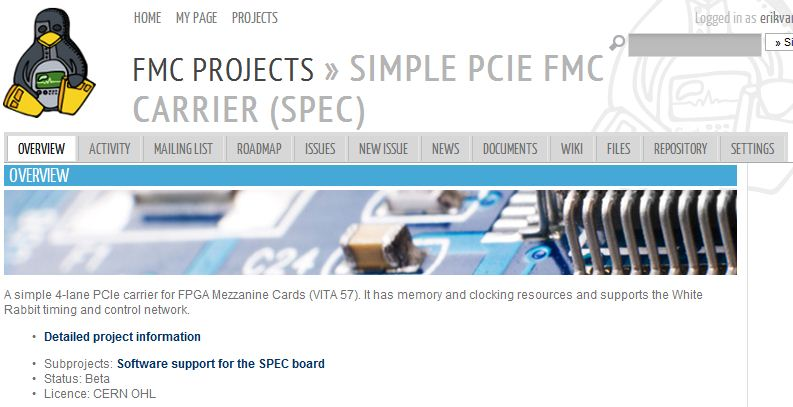
\includegraphics[height=6cm]{ohr_spec_top.jpg}
% \includegraphics[height=6cm]{../pictures/ohwr/EDA-02063-V1-0-TOP1.jpg}% ADC card
%  \includegraphics[height=6cm]{../pictures//BoardBlockDiagramv2.pdf}%
 \end{center} 
\end{frame}

% \iffalse
% \begin{frame}{OHR Status}{October 2011}
%         \begin{block}{Projects}
%    \begin{itemize}
%         \item 46 active projects
%         \begin{itemize}
%     	    \item 38 initiated by CERN groups, 8 by other institutes
%            \end{itemize}
%         \item 3.6 developers on average 
%    \end{itemize}
%         \end{block}
% 
% \begin{block}{Types of designs}
% \begin{itemize}
%         \item About 30 hardware designs (of which 20 FMC projects)
%         \item About 20 re-usable HDL cores
%         \item General tools
%         \begin{itemize}
%     	    \item Production test environment (Python based)
%     	    \item ADC performance test
% %		\item Wishbone slave generator, crossbar
%         \end{itemize}
%    \end{itemize}
%         \end{block}
% \end{frame}
% \fi

\begin{frame}{CERN FMC projects in OHR -- some examples}
\begin{block}{FMC Carriers}
	\begin{itemize}
		\item VME64x, PCIe, AMC, VXS
		\item PXIe in the pipeline
	\end{itemize}
\end{block}

\begin{block}{FMC Mezzanines}
	\begin{itemize}
		\item ADC's, sampling speeds: 200~kSPS, 100~MSPS
		\item TDC and Fine delay (resolution 1 ns)
		\item Digital I/O: 5 channels, 16 channels
	\end{itemize}
\end{block}
\end{frame}

% \begin{frame}{ CERN non-FMC projects in OHR -- some examples}
% \begin{block}{Hardware}
% 	\begin{itemize}
% 		\item TTL to NIM level converter (VME)
% 		\item White Rabbit timing network switch
% 		\item Small footprint ARM-based computer
% 	\end{itemize}
% \end{block}
% \begin{block}{HDL cores, Software and Tools}
% 	\begin{itemize}
% 		\item Wishbone cores: DDR3 controller, VME64x core, serialiser\ldots
% 		\item RISC Processor core
% 		\item Time-to-Digital Converter core
% 		\item NanoFIP WorldFIP interface
% 		\item Production test environment (Python based)
% 	\end{itemize}
% \end{block}
% \end{frame}



% IMAGES non-FMC
% ========
%\begin{frame}{ARMadillo single board ARM-based computer}{runs Linux}
% \begin{center}
%   \includegraphics[height=6cm]{../pictures/ohwr/armadillo.jpg}
% \end{center} 
%\end{frame}


% \begin{frame}{TTL to NIM converter}
%  \begin{center}
%    \includegraphics[height=7cm]{pictures/CVORI_pers.jpg} 
%    \includegraphics[height=7cm]{pictures/CVORI_side.jpg}
%  \end{center} 
% \end{frame}

\subsection{CERN Open Hardware Licence}
%=========================

\begin{frame}{CERN Open Hardware License \href{http://ohwr.org/cernohl}{-- ohwr.org/cernohl}}
	\begin{block}{Provides a solid legal basis}
   \begin{itemize}
	\item Developed with Knowledge Transfer Group at CERN 
	\item Inspired by open software licences
	\item Focused on both design and products
	\item Persistent as LGPL
   \end{itemize}
	\end{block}

\begin{block}{Practical: makes it easier to work with others}
   \begin{itemize}
%	\item Makes it easier to work with others
	\item Upfront clear that anything you give will be available to everyone
	\item Makes it clear that anyone can use it for free
   \end{itemize}
\end{block}
\end{frame}

\begin{frame}{CERN Open Hardware License \href{http://ohwr.org/cernohl}{-- ohwr.org/cernohl}}
	\begin{block}{Same principles as Open Software}
 \begin{itemize}
	 \item Anyone can see the source (design documentation)
	\item Anyone is free to study, modify and share
	\item Any modification and distribution under same licence
	\item Persistence makes everyone profit from improvements
\end{itemize}
	\end{block}

	\begin{block}{Hardware production}
 \begin{itemize}
	\item When produce: licensee is invited to inform the licensor
\end{itemize}
	\end{block}

%
%	\begin{block}{Usage not limited to Open Hardware Repository}
% \begin{itemize}
%	\item Designs outside OHR. Even for mechanical hardware.
%\end{itemize}
%	\end{block}
\end{frame}



%\begin{frame}{CERN Open Hardware License \href{http://ohwr.org/cernohl}{-- ohwr.org/cernohl}}
%\begin{block}{Provides us a solid legal basis}
%   \begin{itemize}
%	\item Makes it easier to work with others
%	\item Upfront clear that anything you give will be available to everyone
%	\item Makes it clear that anyone can use it for free
%   \end{itemize}
%\end{block}
%\begin{block}{Don't give more details here}
%   \begin{itemize}
%	\item See presentation of Myriam Ayass
%   \end{itemize}
%\end{block}
%\end{frame}



%\begin{frame}{CERN Open Hardware License \href{http://ohwr.org/cernohl}{-- ohwr.org/cernohl}}{2/2}
%	\begin{block}{Same principles as Open Software}
% \begin{itemize}
%	 \item Anyone can see the source (design documentation)
%	\item Anyone is free to study, modify and share
%	\item Any modification and distribution under same licence
%	\item Persistence makes everyone profit from improvements
%\end{itemize}
%	\end{block}
%
%	\begin{block}{Hardware production}
% \begin{itemize}
%	\item When produce: licensee is invited to inform the licensor
%\end{itemize}
%	\end{block}
%
%
%	\begin{block}{Usage not limited to Open Hardware Repository}
% \begin{itemize}
%	\item Designs outside OHR. Even for mechanical hardware.
%\end{itemize}
%	\end{block}
%\end{frame}



\begin{frame}{Example of mechanics licenced with the CERN OHL}
 \begin{center}
   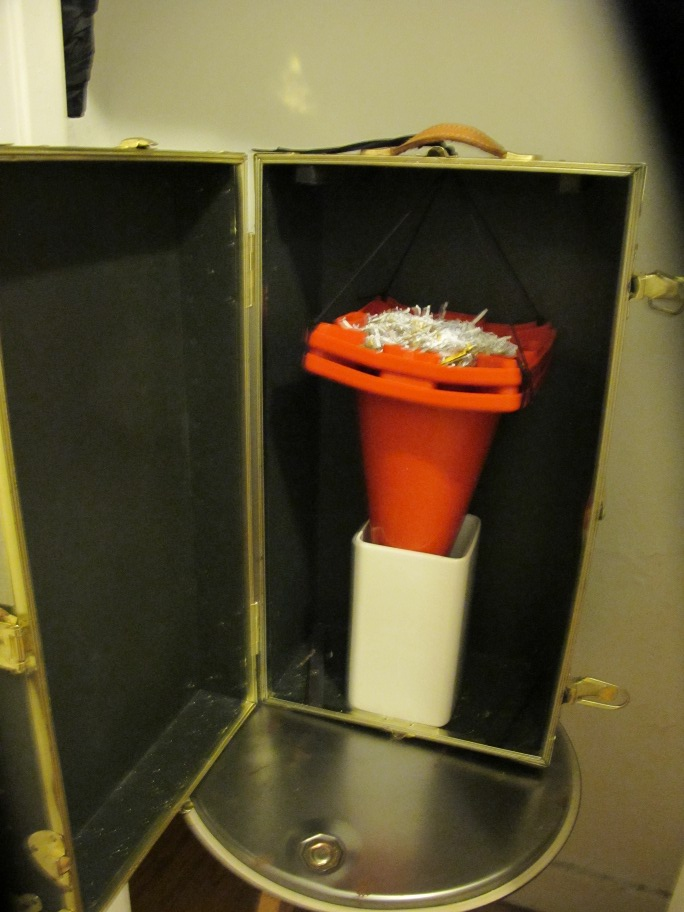
\includegraphics[height=5cm]{worm-farm-008.jpg}
%\hspace{0.3cm}
   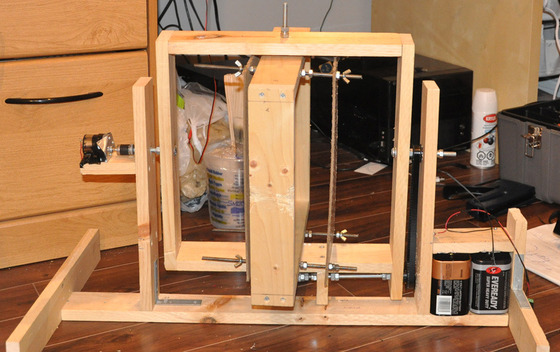
\includegraphics[height=5cm]{rotocaster.jpg}

Worm farm and rotocaster
 \end{center} 
\end{frame}

\begin{frame}{Try to use FOSS tools for development}

\begin{block}{Tools: the last hurdle to sharing}
\begin{itemize}
 \item We already have a forge and a licence.
 \item Current proprietary CAD tools make it hard to share designs.
\end{itemize}
\end{block}

\begin{block}{Current efforts}
\begin{itemize}
 \item Icarus verilog: help in adding VHDL and SystemVerilog support.
 See \href{http://iverilog.icarus.com/}{http://iverilog.icarus.com/}
 \item Kicad: help bring it on par with proprietary tools in terms of
   features and quality. See \href{http://www.ohwr.org/projects/ohr-meta/wiki/Foss-pcb}{http://www.ohwr.org/projects/ohr-meta/wiki/Foss-pcb}.
\end{itemize}
\end{block}

\end{frame}

\section {White Rabbit}

% \frame{\frametitle{Two-way delay compensation schemes}
% \begin{columns}[c]
% \column{1.5in}
% \begin{center}
% 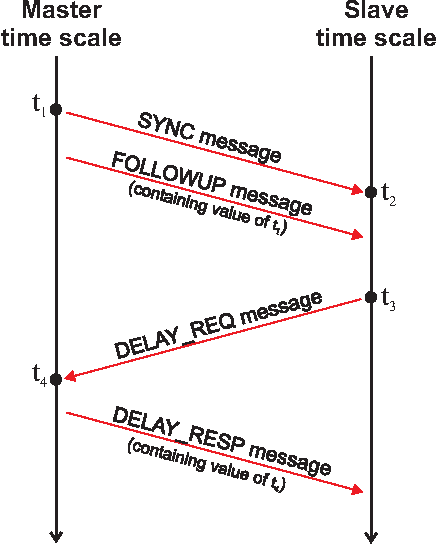
\includegraphics[height=5cm]{ptp_exchange.pdf}
% \end{center}
% \column{2.5in}
% Having the values of $t_{1}$, $t_{2}$, $t_{3}$ and $t_{4}$, the slave can calculate the one-way link delay:\\
% \begin{center} 
% $\delta_{ms} = \frac{(t_{4}-t_{1}) - (t_{3}-t_{2})}{2}$
% \end{center}
% \end{columns}
% }

% \subsubsection{Millisecond timing}

% \frame{
% \frametitle{Millisecond timing clients}
% %\framesubtitle {Hadron therapy}
% \begin{center}
% 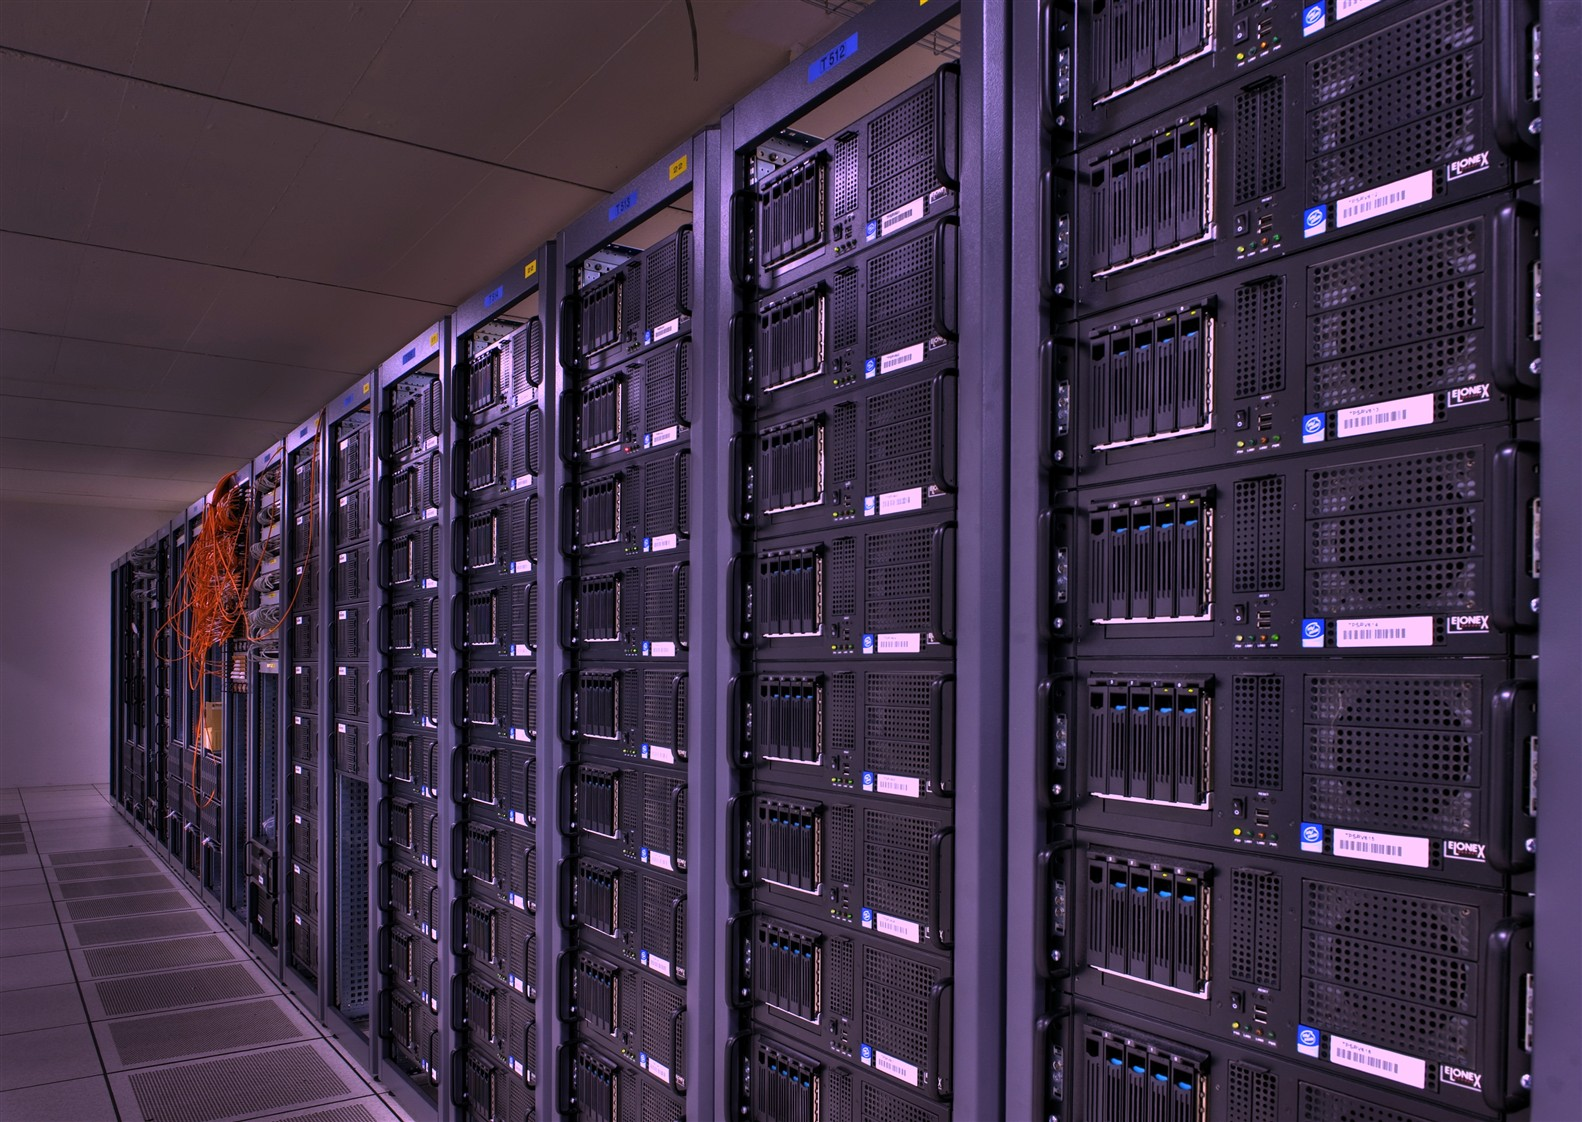
\includegraphics[width=.95\textwidth, height=0.8\textheight, keepaspectratio]{computer_center.jpg}
% \end{center}
% }

% \frame{\frametitle{Millisecond timing}
% \framesubtitle{Example: Network Time Protocol (NTP)}
% \begin{block}{Used in general-purpose computers}
% \begin{itemize}
%   \item Works across the Internet. 
%   \item Each client (slave) gets synchronized to one or more servers.
% \end{itemize}
% \end{block}
% \begin{block}{Cannot do better than 1 ms}
% \begin{itemize}
%   \item Asymmetries in network, switches and routers. 
%   \item Non-determinism due to OS scheduler (time tags done in SW).
%   \item Requires strong statistics artillery to average over many measurements.
% \end{itemize}
% \end{block}
% }

% \subsubsection{Microsecond timing}

% \frame{
% \frametitle{Microsecond timing clients}
% %\framesubtitle {Hadron therapy}
% \begin{center}
% 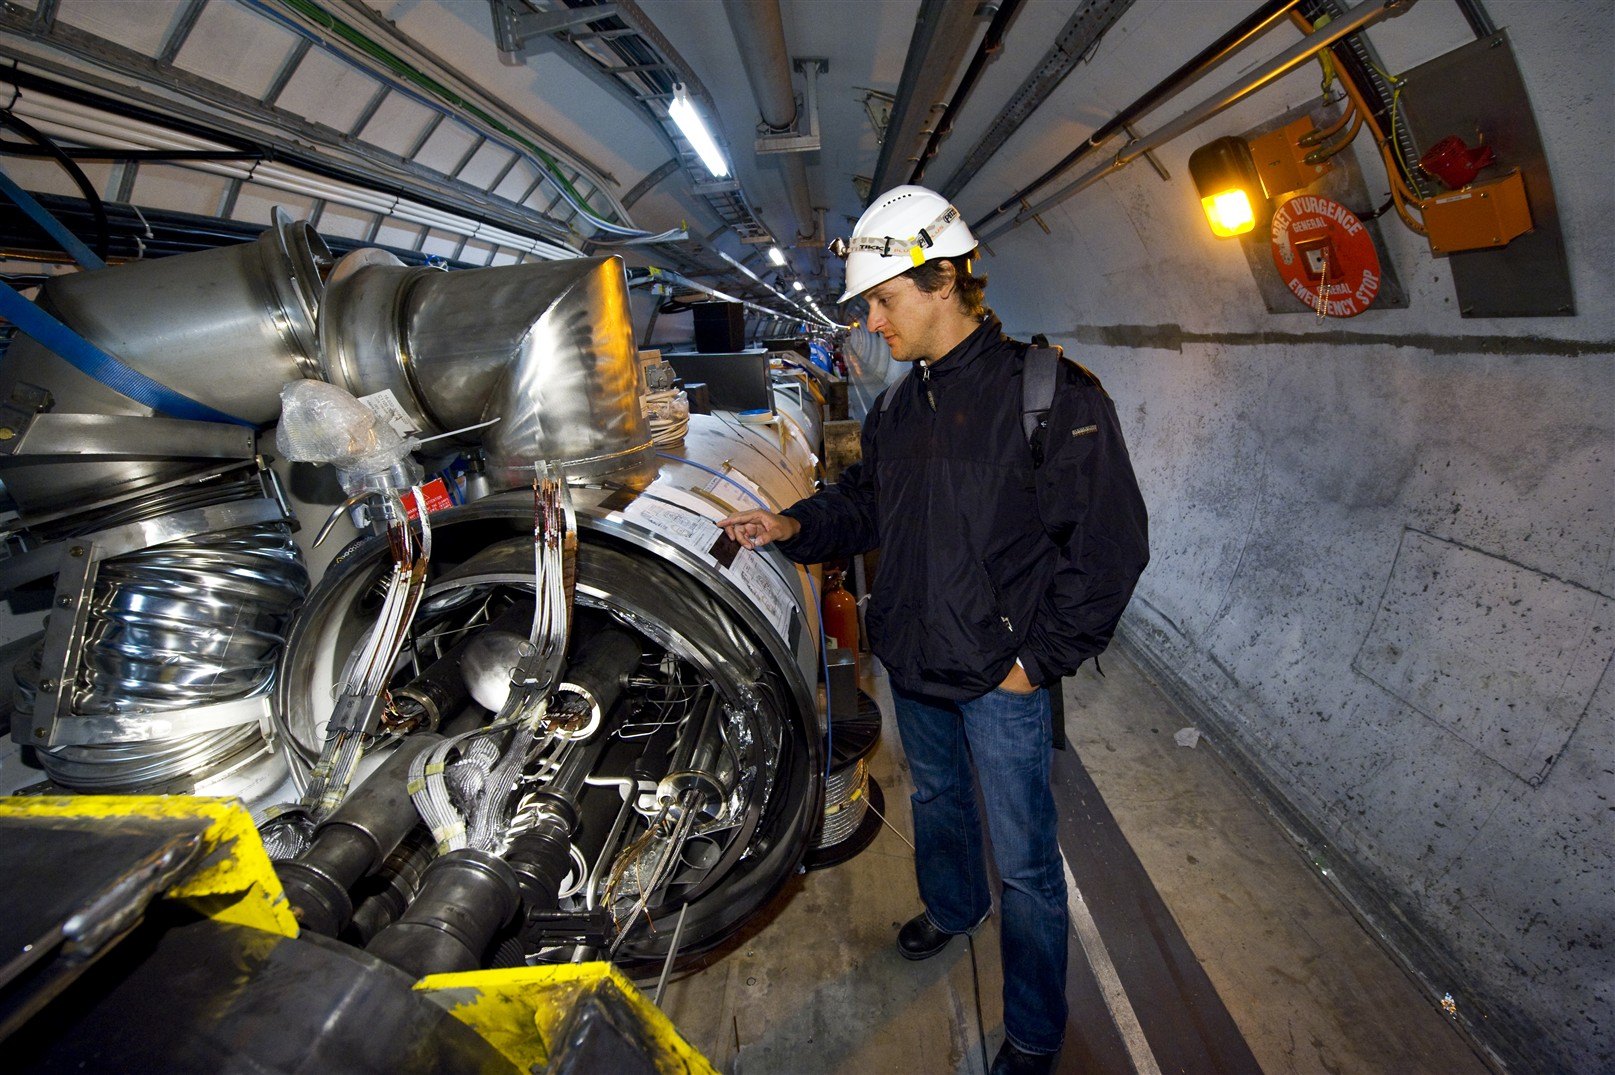
\includegraphics[width=.95\textwidth, height=0.8\textheight, keepaspectratio]{lhc_incident1.jpg}
% \end{center}
% }


% \frame{
% \frametitle{Microsecond timing clients}
% %\framesubtitle {Hadron therapy}
% \begin{center}
% 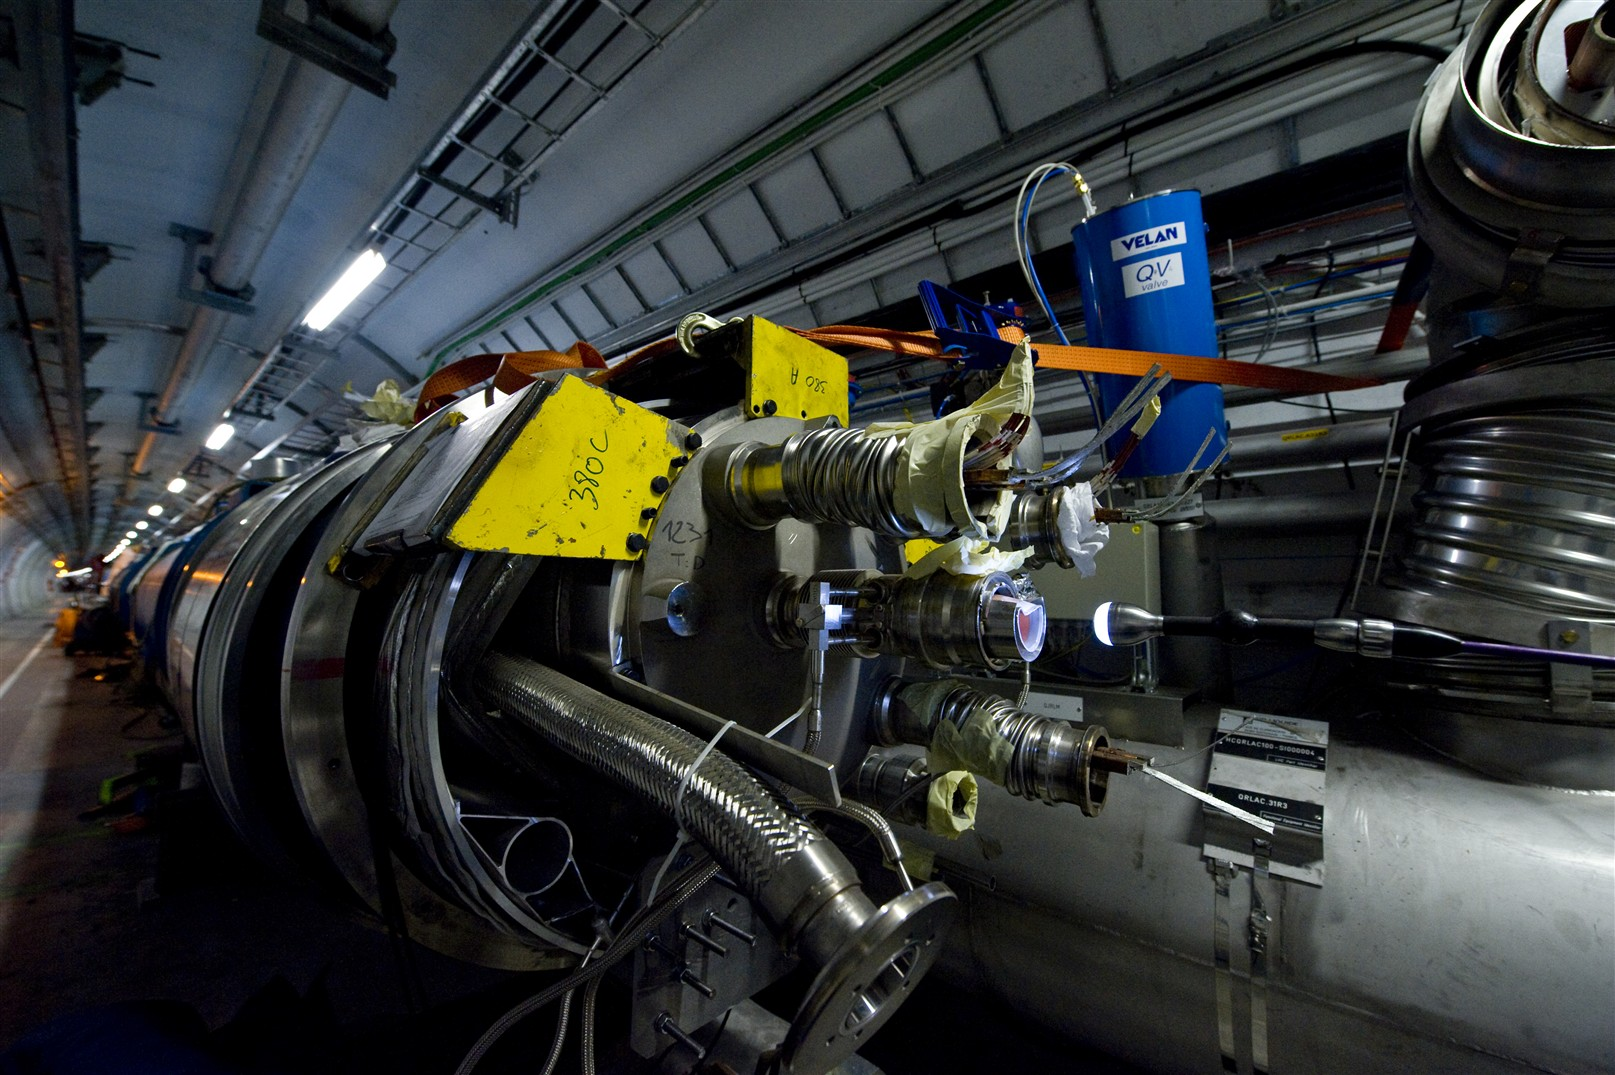
\includegraphics[width=.95\textwidth, height=0.8\textheight, keepaspectratio]{lhc_incident2.jpg}
% \end{center}
% }

% \frame{\frametitle{Microsecond timing}
% \framesubtitle{Example: Precision Time Protocol (PTP, IEEE1588)}
% \begin{block}{Acts on both of NTP's shortcomings}
% \begin{itemize}
%   \item Time-tagging can be done in HW.
%   \item Special PTP switches ensure no loss in precision.
% \end{itemize}
% \end{block}
% \begin{block}{Has a hard time doing better than $1 \mu s$}
% \begin{itemize}
%   \item Typical nodes use a free-running oscillator.
%   \item Frequency offset (and drift) compensation generates extra traffic.
% \end{itemize}
% \end{block}
% }

% \subsubsection{Nanosecond and picosecond timing}

% \frame{
% \frametitle{Nanosecond and picosecond timing clients}
% %\framesubtitle {Hadron therapy}
% \begin{center}
% 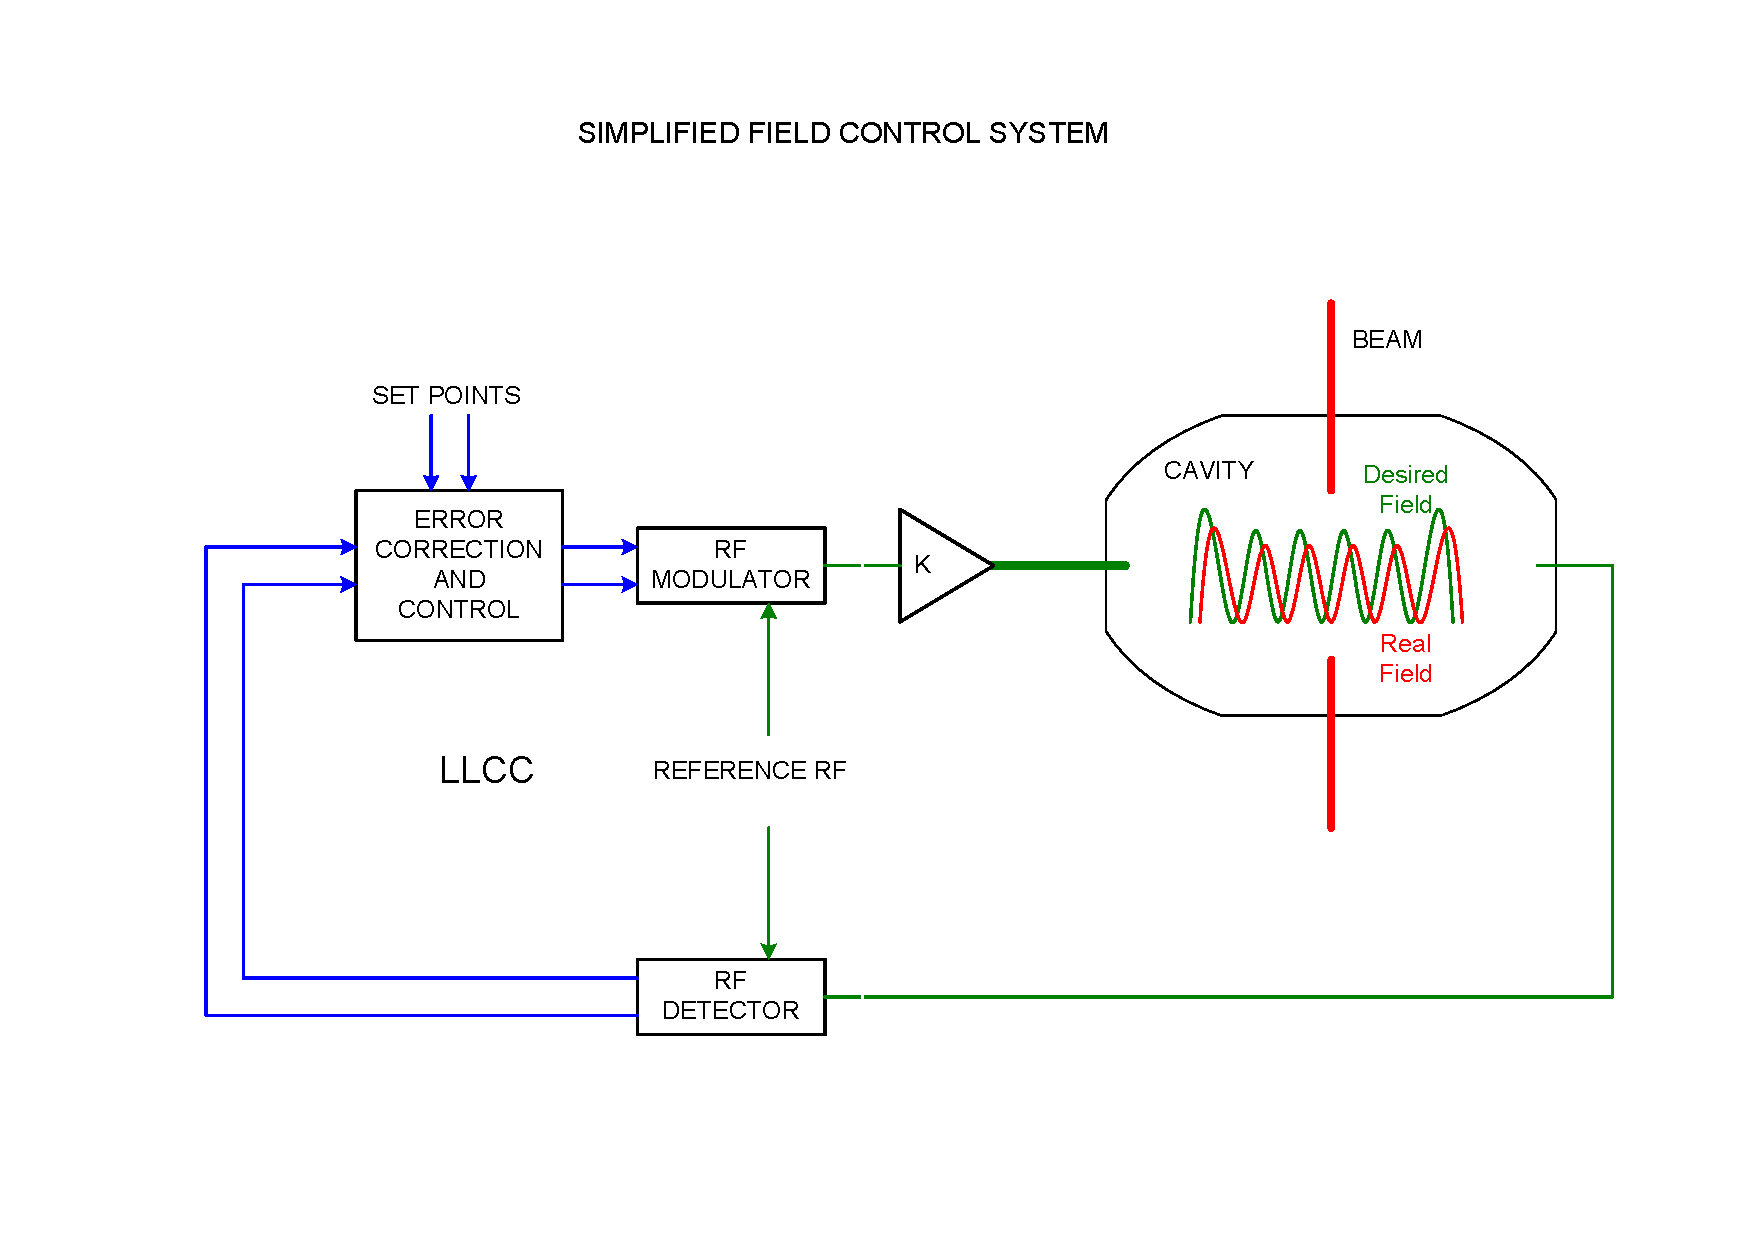
\includegraphics[width=.95\textwidth, height=0.8\textheight, keepaspectratio]{cavity_control.pdf}
% \end{center}
% }

\begin{frame}{What is White Rabbit?}
\begin{center}
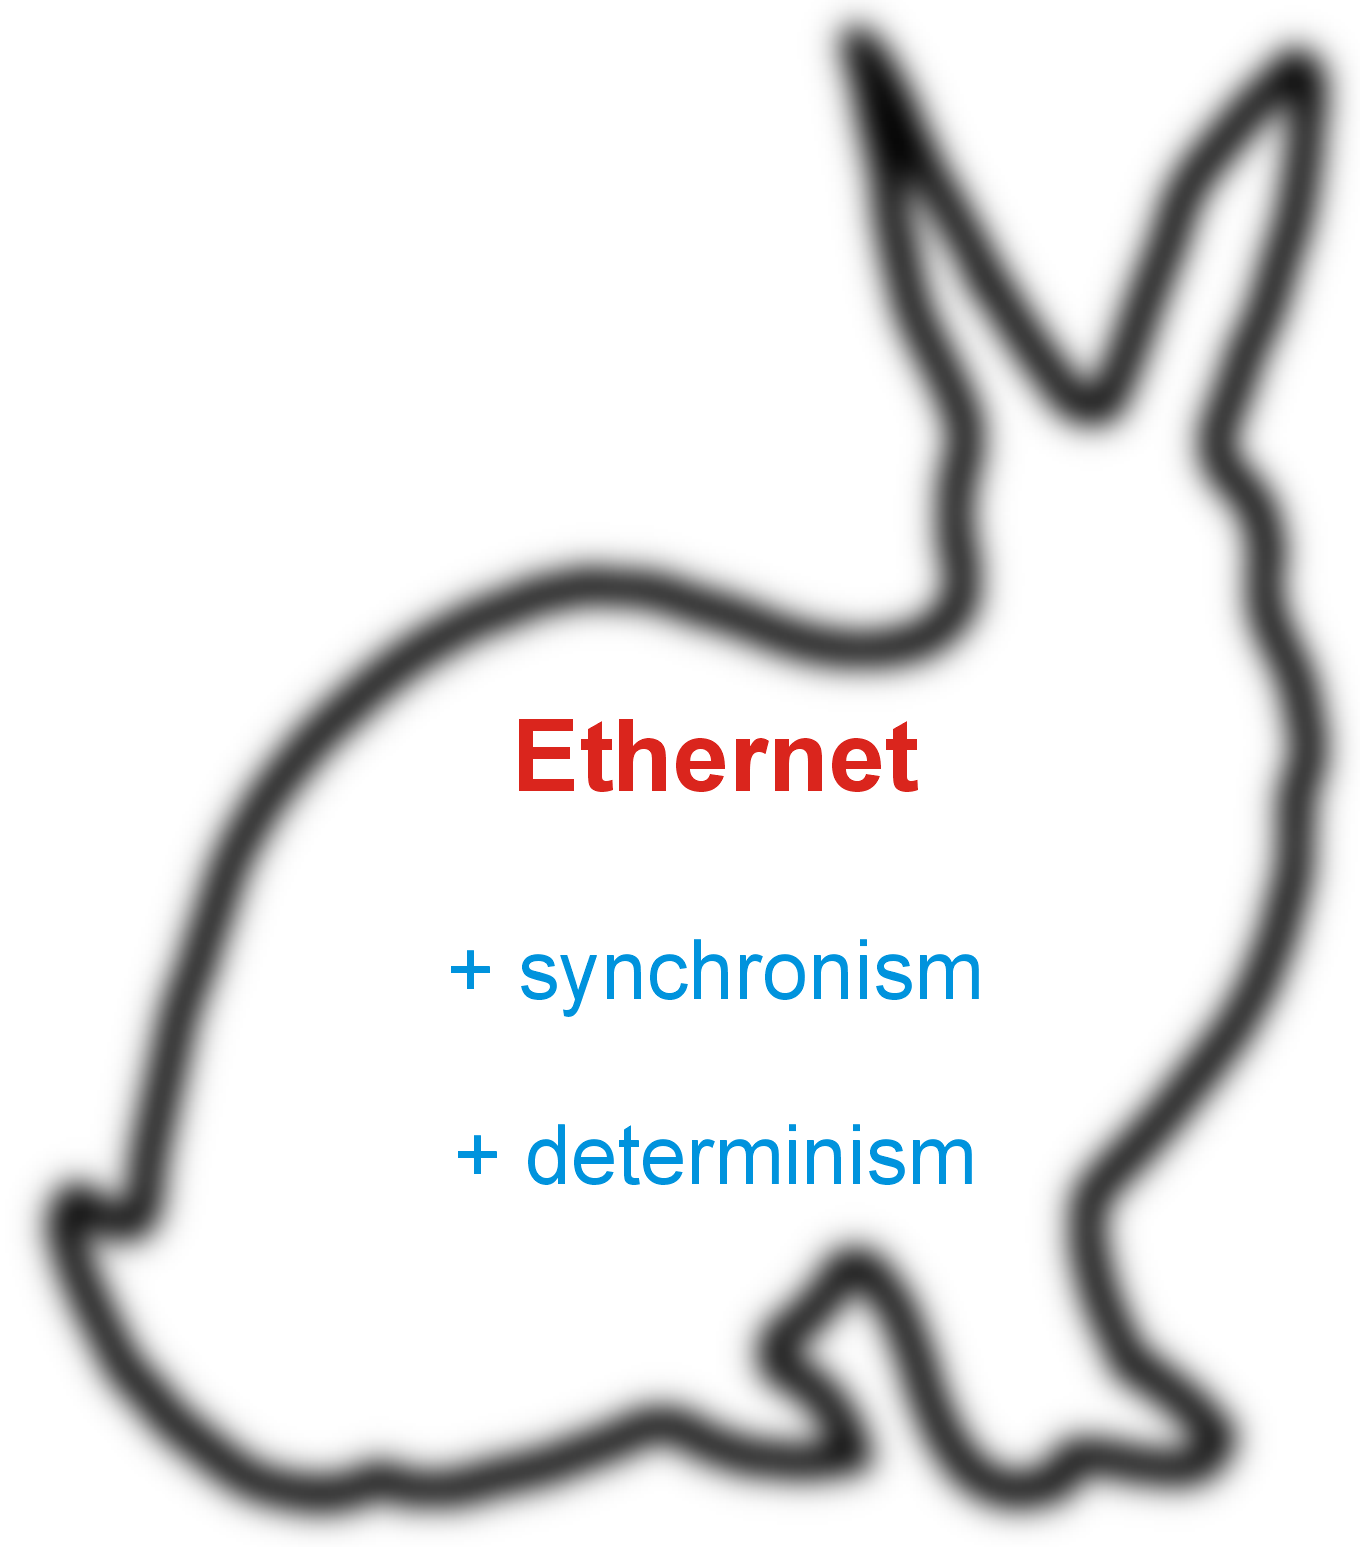
\includegraphics[height=6.5cm]{rabbit.png}
\end{center}
\end{frame}

\frame
{
  \frametitle{What is White Rabbit?}

% Extracting the clock from Ethernet carrier
\begin{block}{}
  An \textbf{extension} to \textbf{Ethernet} which provides:
  \begin{itemize}
% sync mode: - async & sync comparison, tree structure, common clock coming from single source, CDR
% advantage - easy  and precise implementation of time sync
  \item \textbf{Synchronous mode} (Sync-E) - common clock for physical layer in entire network, allowing for precise time and frequency transfer.

\item \textbf{Deterministic routing} latency - a guarantee that packet transmission delay between two stations will never exceed a certain boundary.
\end{itemize}
\end{block}

}

\begin{frame}{Design goals}
\begin{block}{Scalability}
Up to 2000 nodes.
\end{block}

\begin{block}{Range}
10 km fiber links.
\end{block}

\begin{block}{Precision}
1 ns time synchronization accuracy, 20 ps jitter.
\end{block}

\end{frame}

\frame{
\frametitle{White Rabbit Synchronism}
\framesubtitle {General architecture}
\begin{center}
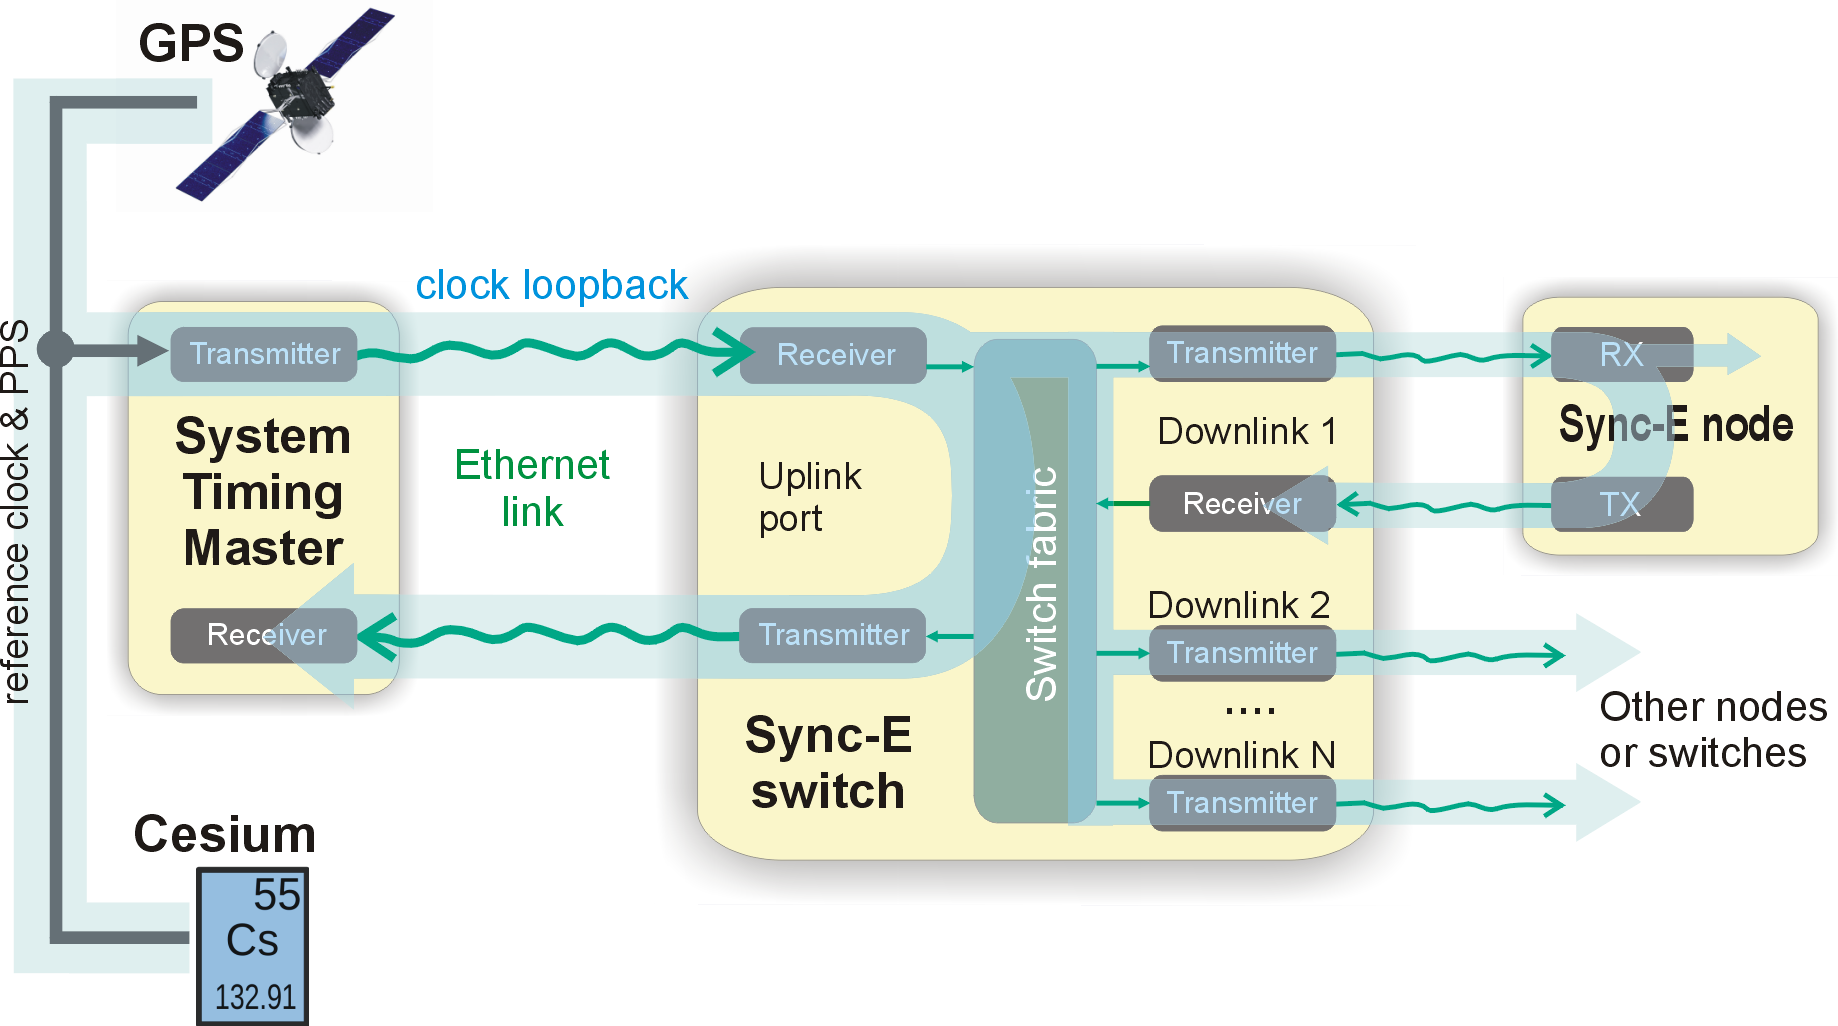
\includegraphics[height=6cm]{synce.png}
\end{center}
}

\frame{
\frametitle{White Rabbit Synchronism}
\framesubtitle {Phase tracking}

\begin{center}
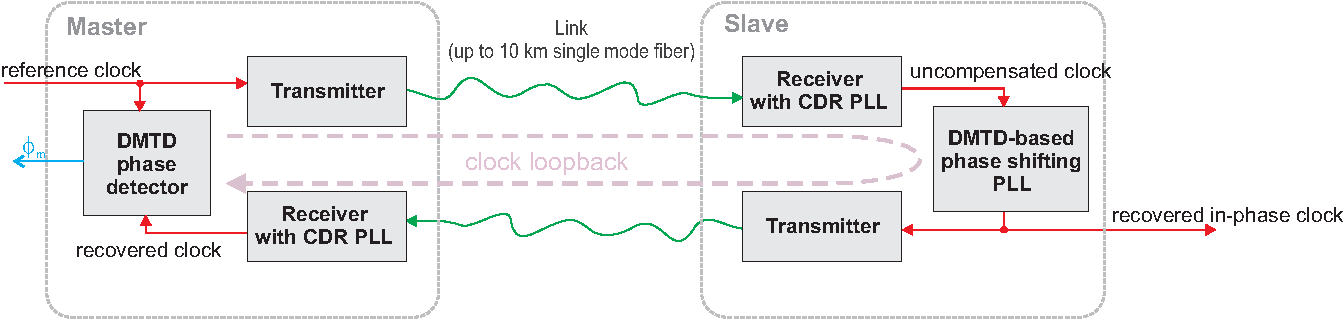
\includegraphics[height=2.5cm]{phase_tracking.pdf}
\end{center}

\begin{itemize}
\item
  Monitor phase of bounced-back clock continuously.
\item
  Phase-locked loop in the slave follows the phase changes measured by the master.
\end{itemize}
}


\begin{frame}{White Rabbit Switch}
\begin{center}
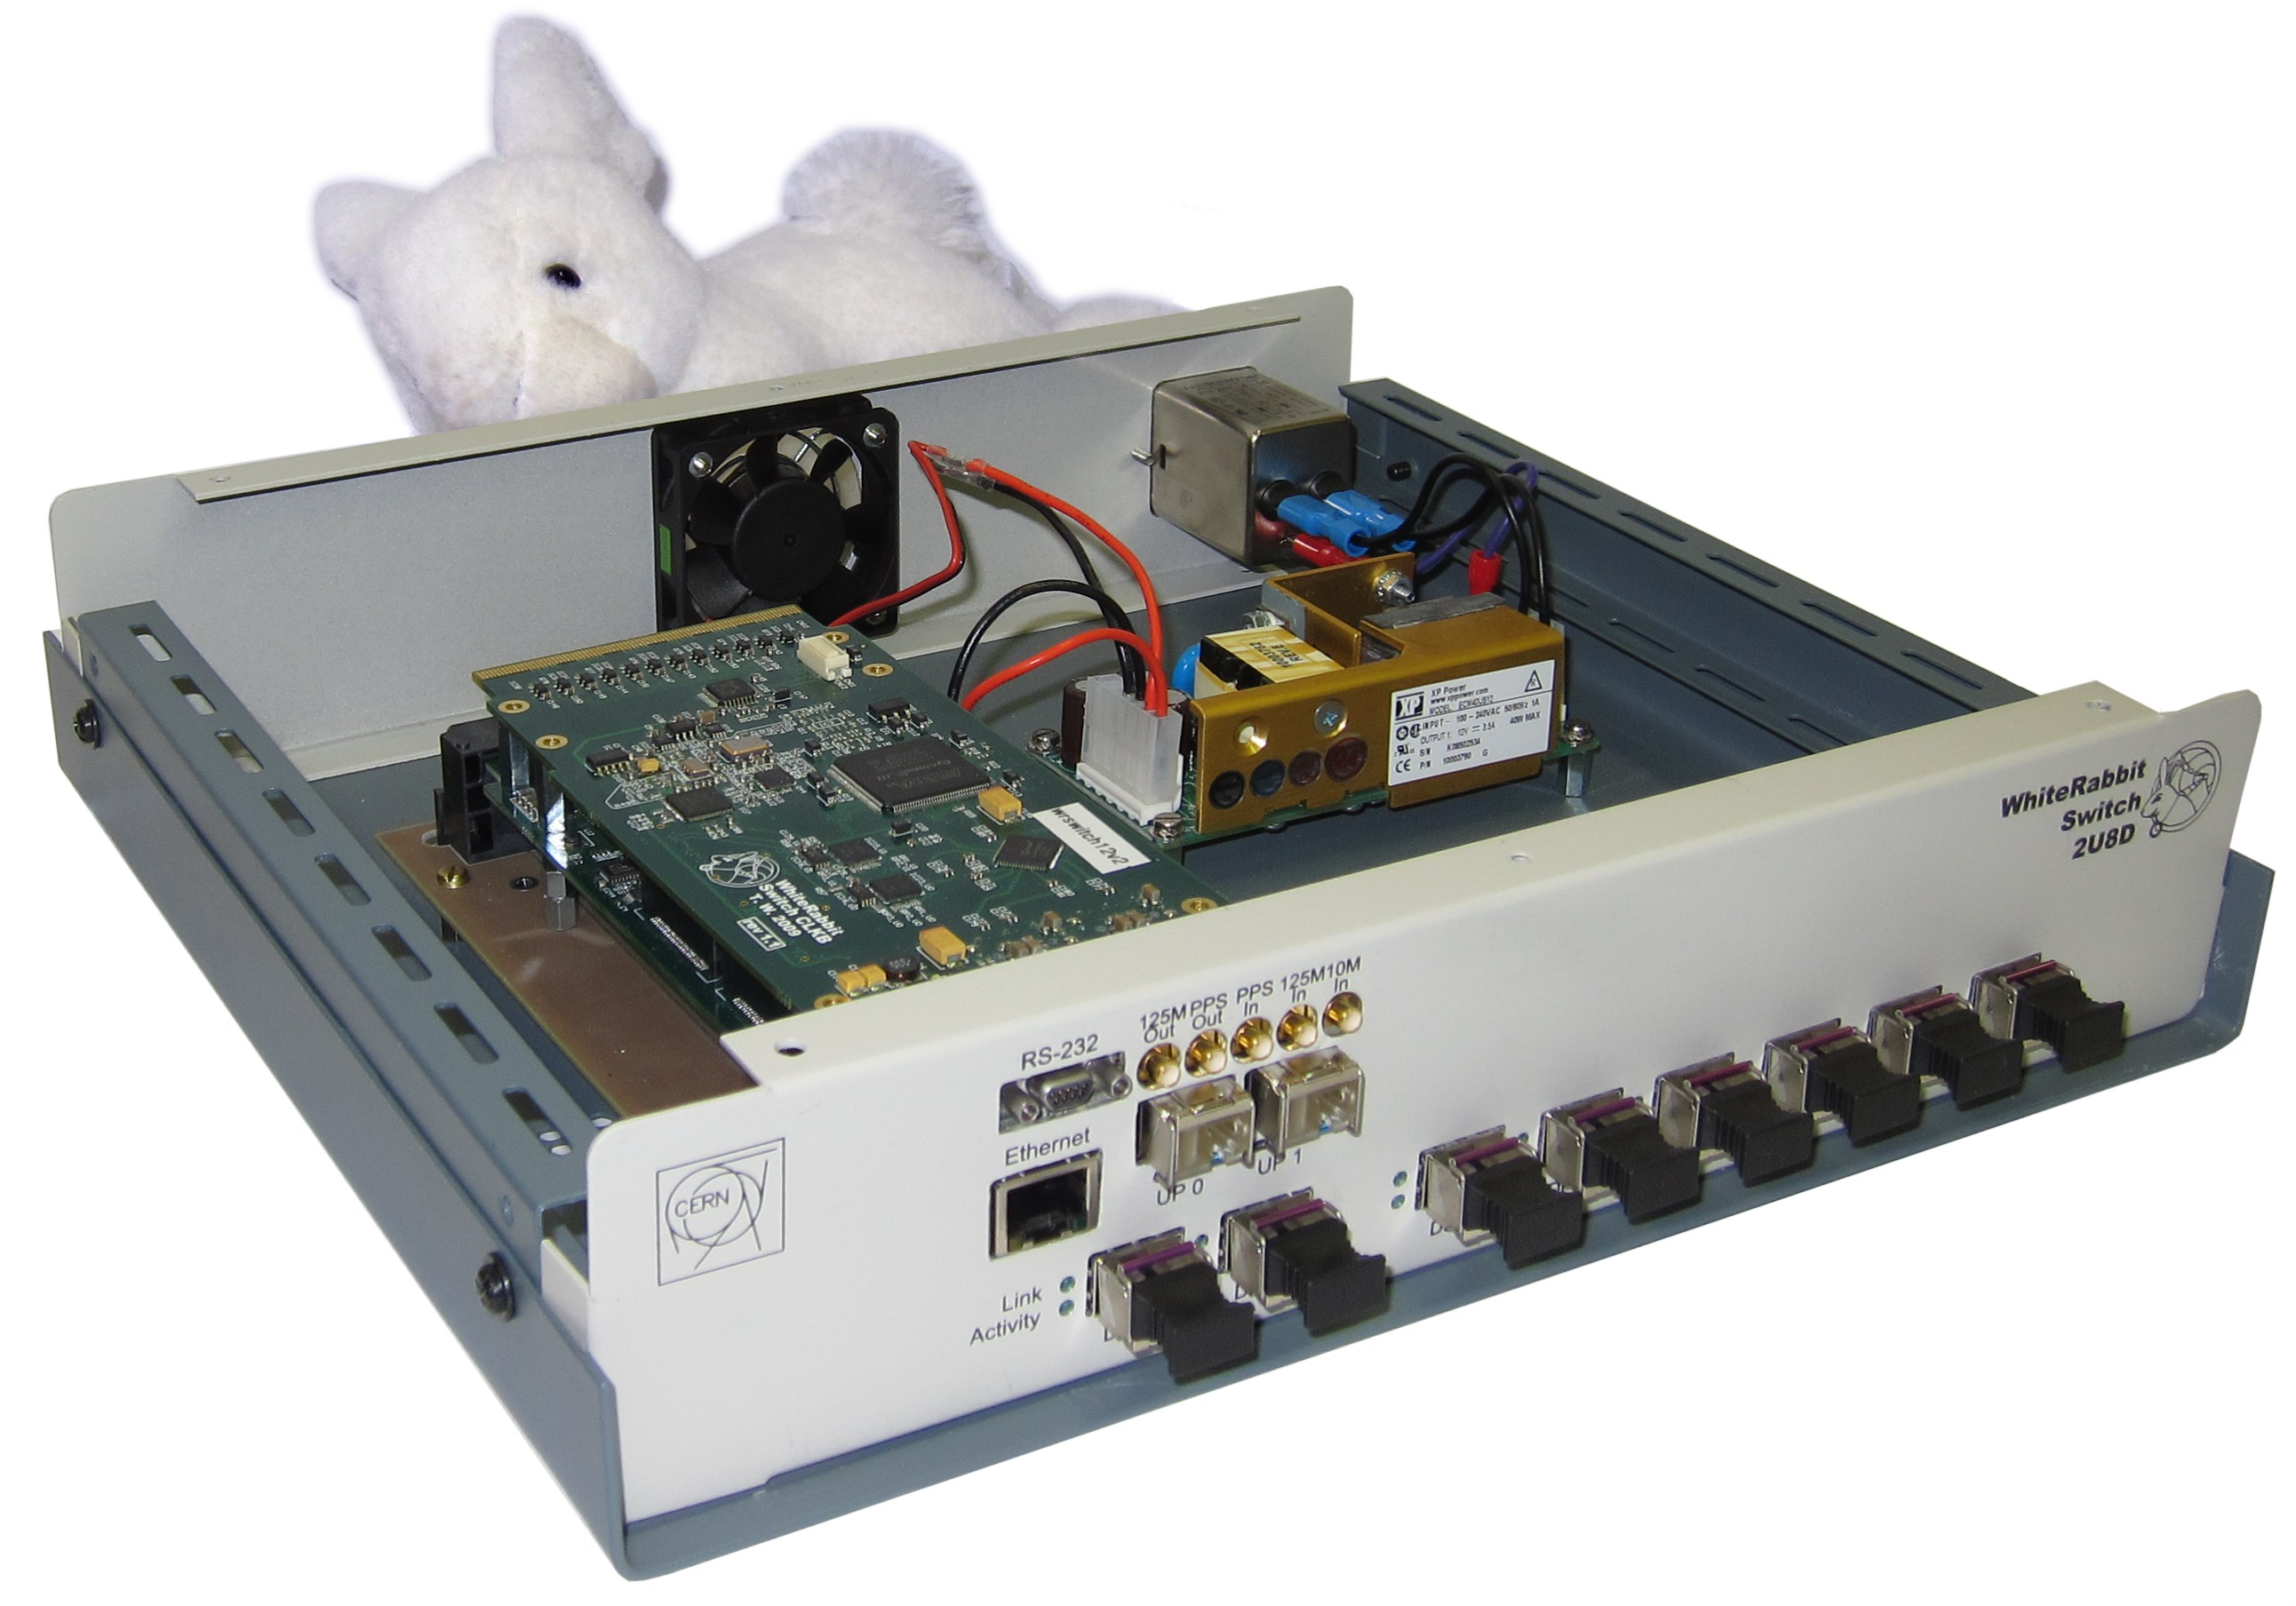
\includegraphics[width=6.5cm]{wrs_photo.jpg}
\end{center}
\begin{itemize}
\item Central element of WR network.
\item Fully custom design, done from scratch at CERN.
\item 10 1000Base-X ports, capable of driving 10+ km of SM fiber.
\item 200 ps synchronization accuracy.
\end{itemize}
\end{frame}

\begin{frame}{Switch block diagram - main part}
\begin{center}
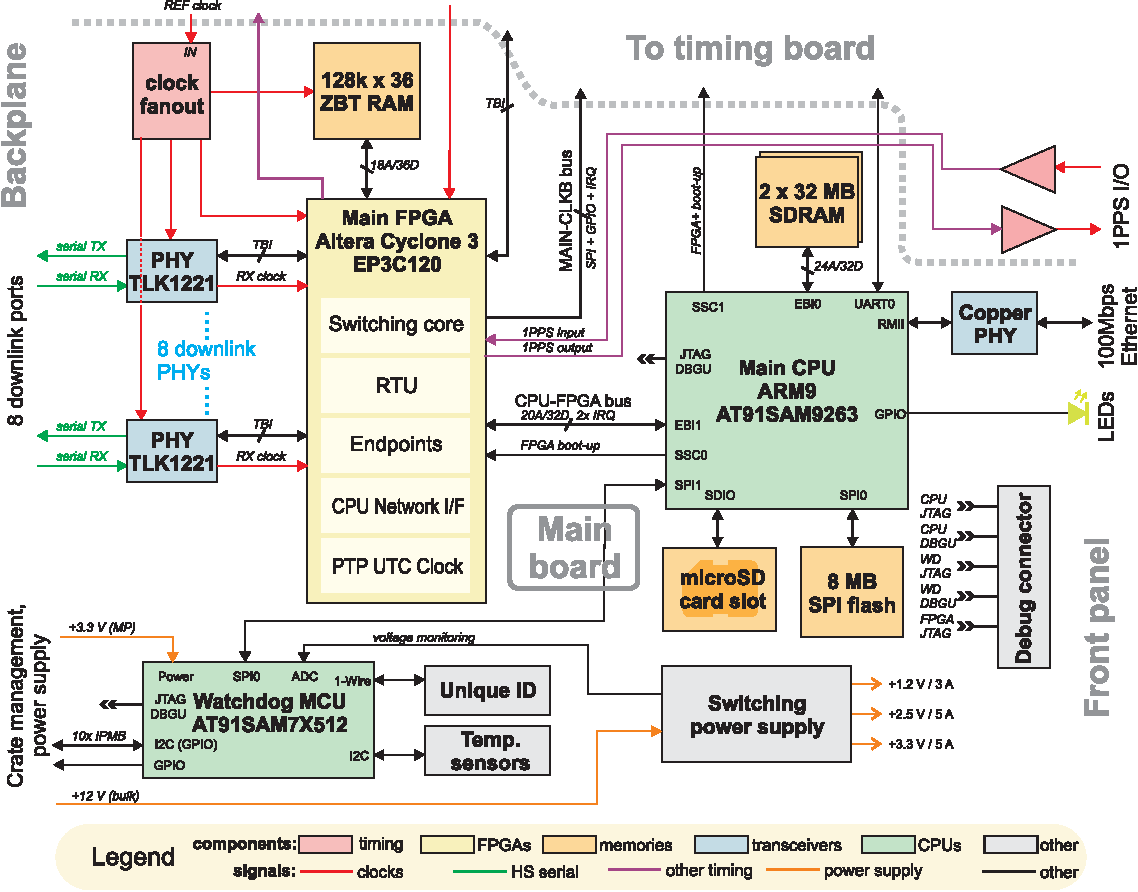
\includegraphics[width=6.5cm]{sw_block.pdf}
\end{center}
\begin{itemize}
\item System FPGA handles all packet processing.
\item Implements PTP stack and management functions (SNMP, Spanning Tree) 
   inside a Linux embedded platform.
\end{itemize}
\end{frame}

\section{Applications}

\subsection{WR in CERN's Hardware Kit}

\begin{frame}{WR in CERN's Hardware Kit}
\begin{center}

  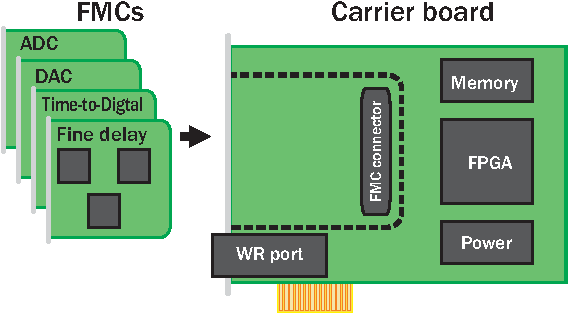
\includegraphics[width=6cm]{shw_kit.pdf}

  \begin{block}{CERN's FMC-based Hardware Kit:}
    \begin{itemize}
    \item FMCs (FPGA Mezzanine Cards) with ADCs, DACs, TDCs, fine delays, digital I/O.
    \item Carrier boards in PCI-Express and VME formats.
    \item All carriers are equipped with a White Rabbit port.
    \end{itemize}
  \end{block}

\end{center}
\end{frame}


% \begin{frame}{Ethernet Clock distribution a.k.a. Distributed DDS}
%   \begin{center}
%     \includegraphics[width=\columnwidth]{drawings/remote_dds.pdf}
%   \end{center}
%   \begin{block}{Distributed Direct Digital Synthesis}
%     \begin{itemize}
%     \item Replaces dozens of cables with a single fiber.
%     \item Works over big distances without degrading signal quality.
%     \item Can provide various clocks (TTC, RF, bunch clock) with a single, standarized link.
%     \end{itemize}
%   \end{block}
% \end{frame}


\begin{frame}{Distributed oscilloscope}
  \begin{center}
    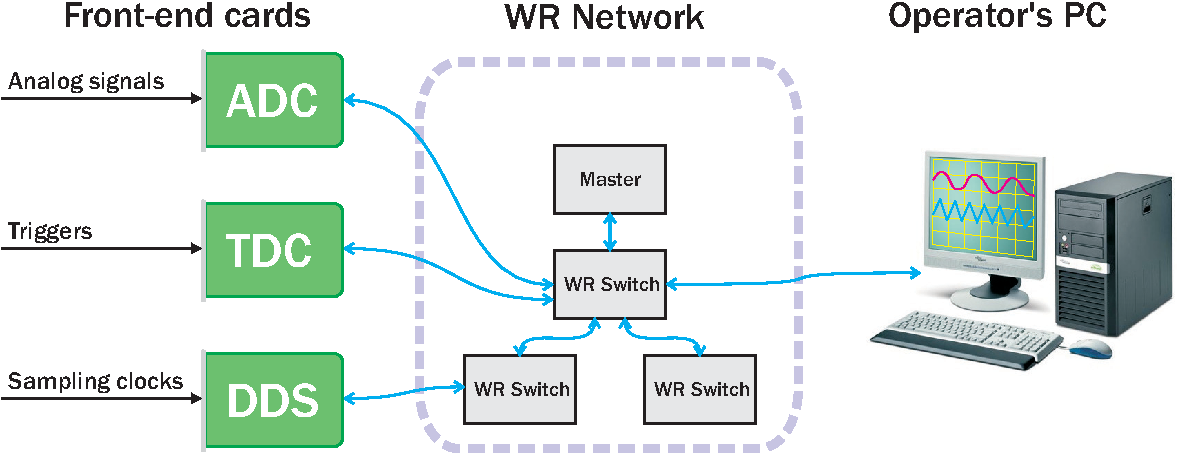
\includegraphics[width=8cm]{distr_oscill.pdf}
    \end{center}
    \begin{block}{}
      \begin{itemize}
      \item Common clock in the entire network: no skew between ADCs.
      \item Ability to sample with different clocks via Distributed DDS.
      \item External triggers can be time tagged with a TDC and used to reconstruct the original time base in the operator's PC.
      \end{itemize}
    \end{block}
\end{frame}



% \frame{
% \frametitle{Nanosecond and picosecond timing}
% \framesubtitle {Another example: neutrino oscillation experiments}
% 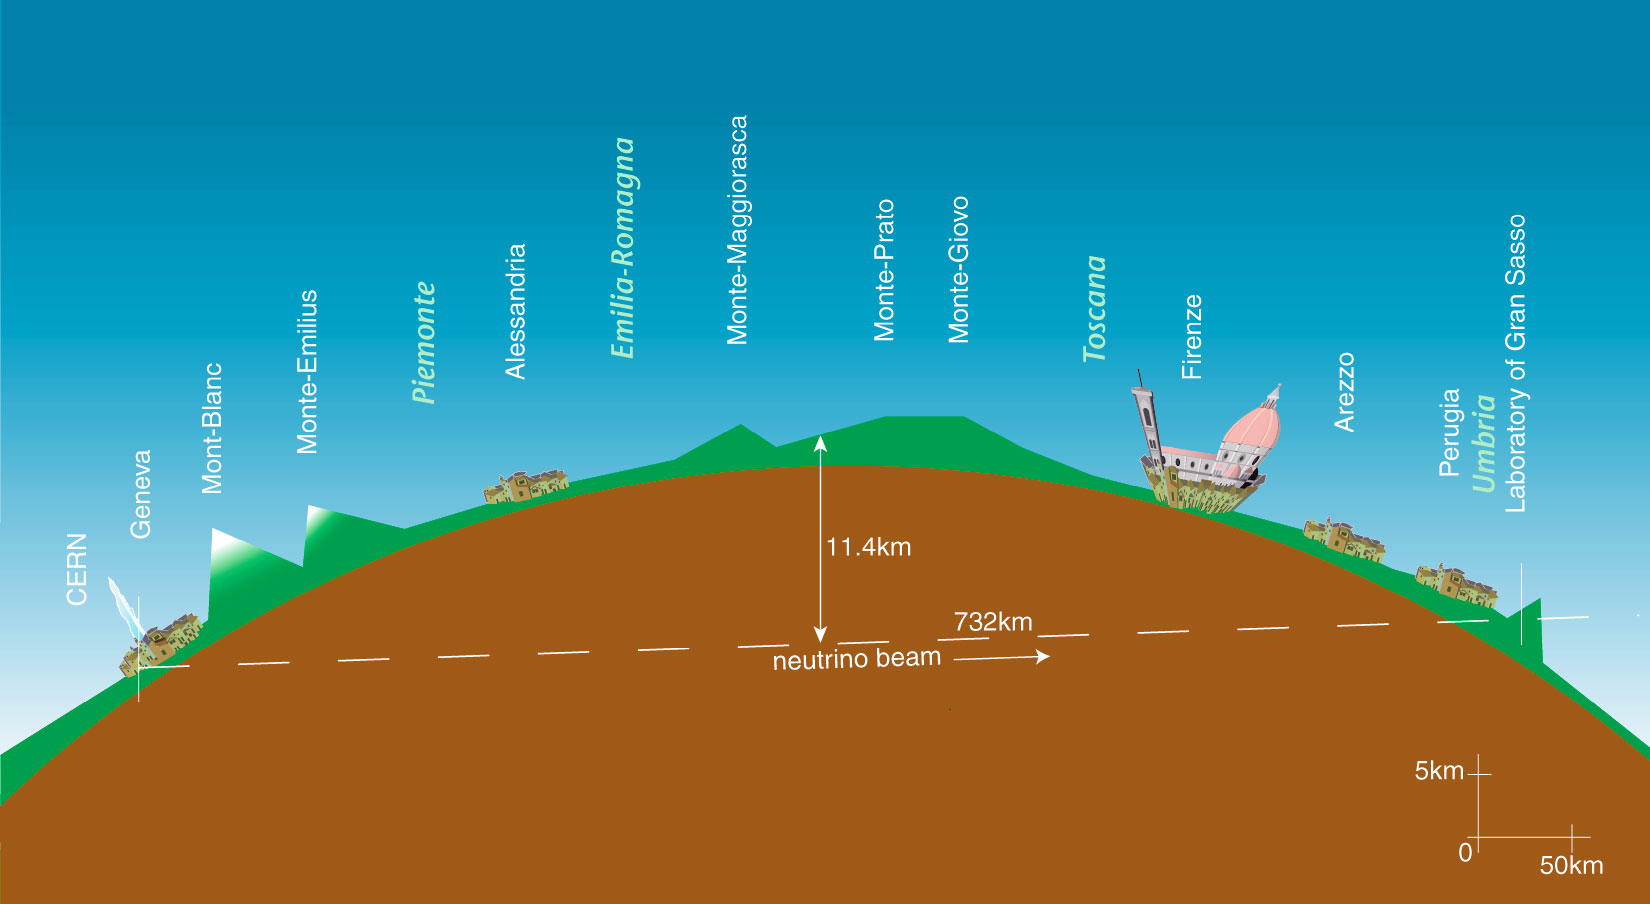
\includegraphics[width=\textwidth]{cern_to_lngs.jpg}
% }

% \frame{
% \frametitle{Nanosecond and picosecond timing}
% \framesubtitle {Another example: neutrino oscillation experiments}
% 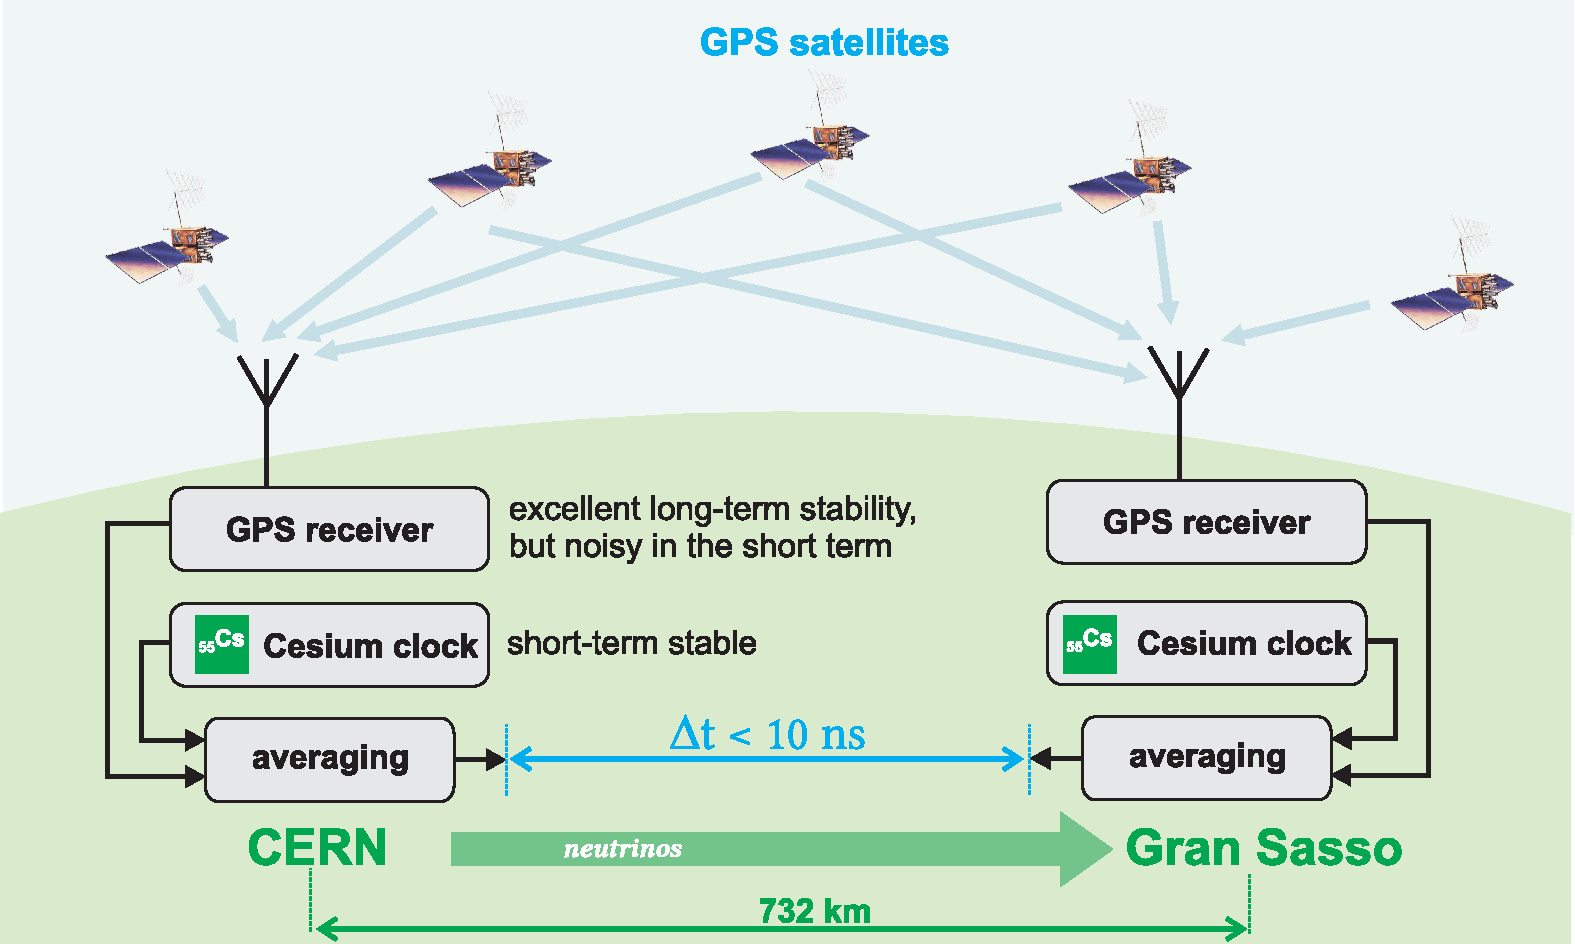
\includegraphics[width=\textwidth]{cern_gransasso.pdf}
% }
%%% \documentclass[compress,red]{beamer}
%%% \usetheme{Warsaw}
%%% \useoutertheme[subsection=false]{smoothbars}
%%% 
%%% \usepackage{helvet}
%%% \usepackage{graphicx}
%%% \usepackage{booktabs}
%%% \usepackage{hyperref}
%%% \usepackage{url}
%%% 
%%% \usepackage{remreset}% tiny package containing just the \@removefromreset command
%%% \makeatletter
%%% \@removefromreset{subsection}{section}
%%% \makeatother
%%% \setcounter{subsection}{1}
%%% 
%%% \title[Managing equipment at CERN]%
%%% 	{A strategy for managing diverse equipment\\
%%% 	in the CERN controls group}
%%% \author[Javier Serrano, David Cobas et al.]{%
%%% 	Javier Serrano, Juan David Gonz\'alez Cobas}
%%% \date{FOSDEM'2012}
%%% 
%%% \begin{document}
%%% 
%%% % ------------------------------------------------------
%%% \begin{frame}
%%% \titlepage
%%% \end{frame}

% ------------------------------------------------------
\section{Software for Diverse Equipment}

\begin{frame}
\frametitle{Software for Diverse Equipment}

We got ourselves a rather diverse hardware ecosyst...
\pause eeehh, sorry, \pause zoo
\pause
\begin{block}{Different species of hardware animals...}
\begin{itemize}
\pause\item analog I/O (ADCs, DACs, waveform generators)
\pause\item digital I/O
\pause\item timing boards (FD, TDC)
\end{itemize}
\end{block}
\pause
\begin{block}{...of diverse breed}
\begin{itemize}
\pause\item legacy stuff
\pause\item FMC boards
\end{itemize}
\end{block}

\pause Some order has to be imposed in the zoo.
\end{frame}

% ------------------------------------------------------
\begin{frame}
\frametitle{Unifying Themes}
\begin{block}{Wishbone-based drivers}
\begin{itemize}
\item covering the FMC family of boards
\item designed around the internal Wishbone bus
\item depending on enumeration of device cores
\end{itemize}
\end{block}
\begin{block}{\texttt{zio}: The Ultimate I/O}
\begin{itemize}
\item Linux kernel framework for I/O devices
\item oriented to high bandwidth applications
\end{itemize}
\end{block}


\end{frame}

\subsection{FMC boards}
% ------------------------------------------------------
\begin{frame}{The FMC family of boards}
\begin{itemize}
\item carriers in PCIe and VME form factors
\item simple mezzanines with electronics for ADCs, DACs, DIO and endless
    other applications
\item circuitry in the mezzanine
\item FPGA application logic in the carrier
\item \emph{logic in the FPGA is organized as a set of IP cores
    interconnected through an internal \textcolor{red}{Wishbone}}
    bus
\end{itemize}
\end{frame}
% ------------------------------------------------------
\begin{frame}{A typical data acquisition application: carrier}
\begin{center}
\includegraphics[height=0.6\textheight]{spec.pdf}
\end{center}
\centering
SPEC carrier board (\url{http://www.ohwr.org/projects/spec})
\end{frame}

% ------------------------------------------------------
\begin{frame}{A typical data acquisition application: mezzanine}
\begin{center}
\includegraphics[rotate=180,height=0.7\textheight]{fmcadc.pdf}
\end{center}
\centering
FMA 100M4ch14b ADC
(\url{http://www.ohwr.org/projects/fmc-adc-100m14b4cha})
\end{frame}

% ------------------------------------------------------
\begin{frame}
\begin{figure}[t]
   \centering
   \includegraphics[width=80mm]{adcarch.pdf}
   \caption{Block diagram of the FMC slow ADC application.}
   \label{slow-adc}
\end{figure}
\end{frame}

% ------------------------------------------------------
\begin{frame}{Parts of the whole}
\begin{itemize}
\item Basic I${}^2$C interfacing to the mezzanine board.
\item Wishbone mastering.
\item DMA access to DDR3 memory in the carrier board.
\item Mezzanine-specific control logic (\emph{e.g.} ADC programming/setup).
\item Interrupt control.
\end{itemize}
\end{frame}

% ------------------------------------------------------
\begin{frame}{Drivers for the FMC family}
The main concepts for the design of these drivers are
\begin{itemize}
\pause
\item modular structure that reflects the core structure of the firmware
\pause
\item one-to-one mapping driver $\leftrightarrow$ core (usually)
\pause
\item ability to dynamically load bitstreams by application
\end{itemize}

\pause
On the whole, the driver for the carrier board acts as a basic firmware
loader and a bridge driver (with device enumeration
\emph{\`a la PCI)} between the host bus (PCIe, VME) and the FPGA
interconnection bus

\pause
It will be (we hope) the first Wishbone bus driver in the mainstream
kernel $\Rightarrow$ will to go upstream, timeliness
\end{frame}


% ------------------------------------------------------
\begin{frame}{Architecture of the FMC drivers}
\includegraphics[height=0.8\textheight]{driverarch.pdf}
\end{frame}

% ------------------------------------------------------
\begin{frame}{How the FMC drivers start up}
\begin{itemize}
\item Identify the carrier board and initialize it.
\item Perform a basic identification of the mezzanine(s) installed in
    the FMC slot(s), and their configured applications.
\item Load the application firmware into the carrier FPGA.
\item Register a Wishbone bus with the kernel.
\item Enumerate the cores in that firmware (to wit, the
    inner blocks in figure~\ref{slow-adc}).
\item Register the devices those cores implement and install the drivers
    associated to them.
\end{itemize}
\end{frame}



\subsection{The \texttt{zio} framework}

% ------------------------------------------------------
\begin{frame}{Industrial I/O frameworks}

\pause
\begin{block}{In Linux staging area}
\begin{itemize}
\item Comedi
\item IIO
\end{itemize}
\end{block}

\pause
\begin{block}{Drawbacks (for CERN applications)}
\begin{itemize}
\item interfaces are cumbersome (Comedi)
\item our use cases are far more complicated
\end{itemize}
\end{block}

\pause
\begin{block}{Then \texttt{zio} comes}
\begin{itemize}
\item Alessandro Rubini and Federico Vaga, main developers
\item Designed \emph{ab initio} for upstream integration
\item See under \url{http://www.ohwr.org/projects/zio}
\end{itemize}
\end{block}

\end{frame}

% ------------------------------------------------------
\begin{frame}
\frametitle{\texttt{zio} features}

The \texttt{zio} framework is designed to flexibly support the following
aspects:
\begin{itemize}
\item Digital and analog input and output.
\item One-shot and streaming (buffered) data acquisition or waveform play.
\item Buffer management and timing for streaming conversion.
\item Resolution.
\item Sampling rate.
\item Timestamping.
\item Calibration, offset and gain.
\item Bit grouping in digital I/O.
\item Triggering of acquisition/output.
\item Support for DMA.
\item Potential to integrate in the main tree.
\end{itemize}

\end{frame}

% ------------------------------------------------------
\begin{frame}
\frametitle{\texttt{zio} concepts}

\begin{block}{\texttt{zio} abstractions}
\begin{description}
\item[devices] victims of our device drivers, contain channels
\item[channels] basic I/O units
\item[channel sets] group channels to be triggered (acquire, output)
	simultaneously
\item[buffers] for input and output buffering, of course
\item[triggers] cause acquisitions to occur
\end{description}
\end{block}

\end{frame}

% ------------------------------------------------------
\begin{frame}
\frametitle{Typical \texttt{zio} input data flow}
\includegraphics[height=0.8\textheight]{flow-temp-in.pdf}
\end{frame}

% ------------------------------------------------------
\begin{frame}
\frametitle{Typical \texttt{zio} output data flow}
\includegraphics[height=0.8\textheight]{flow-temp-out.pdf}
\end{frame}

% ------------------------------------------------------
\begin{frame}{Next candidates for (\texttt{zio}) integration}

And for mainstream integration as well...
\pause
CERN-developed drivers for good old beasts
\begin{itemize}
\pause
\item Struck SIS33xx ADCs
\pause
\item Tews TPCI200/TVME200 carries plus IPOCTAL serial boards
\pause
\item all the CERN BE/CO-supported FMC boards in the Open Hardware Repository
\pause
\item timing receivers, White Rabbit, etc.
\end{itemize}
\end{frame}

\section{Conclusions}

% ------------------------------------------------------
\begin{frame}{Let's summarize}

\begin{itemize}
\pause
\item Accelerator control systems require managing a complex and
    diverse zoo of hardware devices
\pause
\item Open Hardware makes for a much more manageable design and 
    production way
\pause
\item It is proven to work in practice
\pause
\item Both for a big project like White Rabbit and for the myriad
    of heterogeneous devices linked to it
\pause
\item The software side cannot simply live without the Open Software
    model
\pause
\item Especially the Linux kernel! Thanks for the device model and
    the I/O frameworks
\end{itemize}
\end{frame}

\section{Extras}

\subsection {Timing requirements and technologies}

\frame{\frametitle{Two-way delay compensation schemes}
\begin{columns}[c]
\column{1.5in}
\begin{center}
\includegraphics[height=5cm]{ptp_exchange.pdf}
\end{center}
\column{2.5in}
Having the values of $t_{1}$, $t_{2}$, $t_{3}$ and $t_{4}$, the slave can calculate the one-way link delay:\\
\begin{center} 
$\delta_{ms} = \frac{(t_{4}-t_{1}) - (t_{3}-t_{2})}{2}$
\end{center}
\end{columns}
}

\subsubsection{Millisecond timing}

\frame{
\frametitle{Millisecond timing clients}
%\framesubtitle {Hadron therapy}
\begin{center}
\includegraphics[width=.95\textwidth, height=0.8\textheight, keepaspectratio]{computer_center.jpg}
\end{center}
}

\frame{\frametitle{Millisecond timing}
\framesubtitle{Example: Network Time Protocol (NTP)}
\begin{block}{Used in general-purpose computers}
\begin{itemize}
  \item Works across the Internet. 
  \item Each client (slave) gets synchronized to one or more servers.
\end{itemize}
\end{block}
\begin{block}{Cannot do better than 1 ms}
\begin{itemize}
  \item Asymmetries in network, switches and routers. 
  \item Non-determinism due to OS scheduler (time tags done in SW).
  \item Requires strong statistics artillery to average over many measurements.
\end{itemize}
\end{block}
}

\subsubsection{Microsecond timing}

\frame{
\frametitle{Microsecond timing clients}
%\framesubtitle {Hadron therapy}
\begin{center}
\includegraphics[width=.95\textwidth, height=0.8\textheight, keepaspectratio]{lhc_incident1.jpg}
\end{center}
}


\frame{
\frametitle{Microsecond timing clients}
%\framesubtitle {Hadron therapy}
\begin{center}
\includegraphics[width=.95\textwidth, height=0.8\textheight, keepaspectratio]{lhc_incident2.jpg}
\end{center}
}

\frame{\frametitle{Microsecond timing}
\framesubtitle{Example: Precision Time Protocol (PTP, IEEE1588)}
\begin{block}{Acts on both of NTP's shortcomings}
\begin{itemize}
  \item Time-tagging can be done in HW.
  \item Special PTP switches ensure no loss in precision.
\end{itemize}
\end{block}
\begin{block}{Has a hard time doing better than $1 \mu s$}
\begin{itemize}
  \item Typical nodes use a free-running oscillator.
  \item Frequency offset (and drift) compensation generates extra traffic.
\end{itemize}
\end{block}
}

\subsubsection{Nanosecond and picosecond timing}

\frame{
\frametitle{Nanosecond and picosecond timing clients}
%\framesubtitle {Hadron therapy}
\begin{center}
\includegraphics[width=.95\textwidth, height=0.8\textheight, keepaspectratio]{cavity_control.pdf}
\end{center}
}

\frame{
\frametitle{Nanosecond and picosecond timing}
\framesubtitle {Example: White Rabbit}
\begin{center}
\includegraphics[height=6cm]{synce.png}
\end{center}
}

\frame{
\frametitle{Nanosecond and picosecond timing}
\framesubtitle {Phase tracking}

\begin{center}
\includegraphics[height=2.5cm]{phase_tracking.pdf}
\end{center}

\begin{itemize}
\item
  Monitor phase of bounced-back clock continuously.
\item
  Phase-locked loop in the slave follows the phase changes measured by the master.
\end{itemize}
}

\frame{
\frametitle{Nanosecond and picosecond timing}
\framesubtitle {Another example: neutrino oscillation experiments}
\includegraphics[width=\textwidth]{cern_to_lngs.jpg}
}

\frame{
\frametitle{Nanosecond and picosecond timing}
\framesubtitle {Another example: neutrino oscillation experiments}
\includegraphics[width=\textwidth]{cern_gransasso.pdf}
}

%%% \end{document}
\end{document}

